%% ----------------------------------------------------------------
%% Thesis.tex -- MAIN FILE (the one that you compile with LaTeX) XD
%% ---------------------------------------------------------------- 

% Set up the document
\documentclass[a4paper, 11pt, oneside]{Thesis}
  % Use the "Thesis" style, based on the ECS Thesis style by Steve Gunn

% Include any extra LaTeX packages required
\usepackage[square, numbers, comma, sort&compress]{natbib}  % Use the "Natbib" style for the references in the Bibliography
\usepackage{verbatim}  % Needed for the "comment" environment to make LaTeX comments
\usepackage{vector}  % Allows "\bvec{}" and "\buvec{}" for "blackboard" style bold vectors in maths
\hypersetup{urlcolor=black, colorlinks=false}  % Colours hyperlinks in blue, but this can be distracting if there are many links.
\usepackage{float}
\floatstyle{plaintop}
\restylefloat{table}

\usepackage{csquotes}
\usepackage[T1]{fontenc}
\usepackage[scaled=0.85]{beramono}
\usepackage{listings}
\usepackage{tikz}
\usepackage{3dplot}
\usepackage{tabularx}
\usepackage{lipsum}
\usetikzlibrary{plotmarks}
\usepackage{pgfplots}
\pgfplotsset{compat=1.8}
\usepackage{eurosym}      %<-- For EURO symbol 
\usepackage{filecontents} 
\lstset{basicstyle=\ttfamily,
	showstringspaces=false,
	commentstyle=\color{red},
	keywordstyle=\color{blue}
}
\usepackage{url}

\usepackage[utf8]{inputenc}
%\usepackage[english]{babel}
\usepackage{amssymb}
\usepackage{url}
\usepackage{hyperref}
\usepackage{todonotes}
\usepackage{comment}
\usepackage{pifont}
\usepackage{amssymb}
\setcounter{tocdepth}{3}
\usepackage{graphicx}
\graphicspath{ {images/} }
\usepackage{amsmath}
\usepackage{algorithm2e}
\usepackage{listings}
\usepackage{afterpage}
%\newcommand{\todo}[1]{{\sl\color{red}$\mathcal{TODO}$: #1}}

\usepackage{spverbatim}
\usepackage{fancyvrb}
\fvset{fontsize=\footnotesize}
\let\verb\Verb

\usepackage{paralist}
\newcolumntype{C}[1]{>{\centering}m{#1}}
\newcommand{\prop}[1]{{\verb|#1|}}

\newcommand{\wikidata}{{Sentiment Analysis}\xspace}
\newcommand{\dbpedia}{{DBpedia}\xspace}
\newcommand{\DW}{{\scshape DBw}\xspace}
\newcommand{\rdf}{{RDF}\xspace}

\renewcommand*{\sectionautorefname}{Section}
\renewcommand*{\subsectionautorefname}{Section}
\renewcommand*{\subsubsectionautorefname}{Section}
\newcommand\blankpage{%
	\null
	\thispagestyle{empty}%
	\addtocounter{page}{-1}%
	\newpage}

\usepackage{fancyhdr}
%% ----------------------------------------------------------------
\begin{document}

\frontmatter      % Begin Roman style (i, ii, iii, iv...) page numbering

% Set up the Title Page
\title  {Entity Based Sentiment Classifier for Social Media Analysis}
\authors  {\texorpdfstring
            {{Cristobal Leiva}}
            {Cristobal Leiva}
            }
\addresses  {\groupname\\\deptname\\\univname}  % Do not change this here, instead these must be set in the "Thesis.cls" file, please look through it instead
\date       {\today}
\subject    {}
\keywords   {Machine Learning, SVM, Sentiment Analysis, NLP, IR}

\maketitle
%% ----------------------------------------------------------------

\setstretch{1.3}  % It is better to have smaller font and larger line spacing than the other way round

% Define the page headers using the FancyHdr package and set up for one-sided printing
  % Clears all page headers and footers
\rhead{\thepage}  % Sets the right side header to show the page number
  % Clears the left side page header

\pagestyle{fancy}  % Finally, use the "fancy" page style to implement the FancyHdr headers

%% ----------------------------------------------------------------
% Declaration Page required for the Thesis, your institution may give you a different text to place here
\Declaration{

% \addtocontents{toc}{\vspace{1em}}  % Add a gap in the Contents, for aesthetics


I, Cristobal Leiva, declare that this thesis titled, 'Entity based Sentiment Classifier for Social Media Analysis' and the work presented in it are my own. I confirm that:

\begin{itemize} 
\item This work was done wholly or mainly while in candidature for a research degree at this University.
\item Where any part of this thesis has previously been submitted for a degree or any other qualification at this University or any other institution, this has been clearly stated.
\item Where I have consulted the published work of others, this is always clearly attributed.
\item Where I have quoted from the work of others, the source is always given. With the exception of such quotations, this thesis is entirely my own work.
\item I have acknowledged all main sources of help.
\end{itemize}

Cristobal Leiva
  
Signed:\\
\rule[1em]{25em}{0.5pt}  % This prints a line for the signature
 
Date:\\
\rule[1em]{25em}{0.5pt}  % This prints a line to write the date
}
\clearpage  % Declaration ended, now start a new page

%--------------------------------------------------------------

%% ----------------------------------------------------------------
% The "Quote Page"
\pagestyle{empty}  % No headers or footers for the following pages

\null\vfill
% Now comes the "Funny Quote", written in italics
\textit{"Achievement of your happiness is the only moral purpose of your life, and that happiness, not pain or mindless self-indulgence, is the proof of your moral integrity, since it is the proof and the result of your loyalty to the achievement of your values."}

\begin{flushright}
	Ayn Rand (1905-1982), American philosopher.
\end{flushright}

\vfill\vfill\vfill\vfill\vfill\vfill\null
\clearpage  %Quote page ended, start a new page
%% ----------------------------------------------------------------

% The Acknowledgements page, for thanking everyone
\clearpage  % End of the Acknowledgements
\afterpage{\blankpage}
%% ----------------------------------------------------------------

\pagestyle{fancy}  %The page style headers have been "empty" all this time, now use the "fancy" headers as defined before to bring them back


%% ----------------------------------------------------------------
%\lhead{\emph{Contents}}  % Set the left side page header to "Contents"
\tableofcontents  % Write out the Table of Contents

%% ----------------------------------------------------------------
%\lhead{\emph{List of Figures}}  % Set the left side page header to "List of Figures"
\listoffigures  % Write out the List of Figures

%% ----------------------------------------------------------------
%\lhead{\emph{List of Tables}}  % Set the left side page header to "List of Tables"
\listoftables  % Write out the List of Tables

%% ----------------------------------------------------------------
%\lhead{\emph{List of Listings}}  % Set the left side page header to "List of Listings"
%\lstlistoflistings  % Write out the List of Listings

%% ----------------------------------------------------------------
\mainmatter	  % Begin normal, numeric (1,2,3...) page numbering


% The Abstract Page
%\addtotoc{Abstract}  % Add the "Abstract" page entry to the Contents
\abstract{
	% \addtocontents{toc}{\vspace{1em}}  % Add a gap in the Contents, for aesthetics
	
	
	Having a notion of people’s opinions has always been an essential asset for the decision-making processes in many business models. Therefore, the popularity of sentiment analysis of social media content has being growing rapidly in the last years. However, state-of-the-art sentiment classification approaches lack the capability of performing entity-based classification to identify opinion expressions targeting a specific term, word or entity. In this thesis, this particular problem of entity-based sentiment classification is addressed. 
	
	Combining machine learning and natural language processing methods, the solution proposed in this project uses several sentiment analysis techniques such as Named Entity Recognition (NER), POS tagging, feature vector generation, bag-of-words model and others. These are required to train a Support Vector Machine that classifies tweets (from Twitter) as positive, negative or neutral based on sentiments expressed toward a given target entity (company, person or product). Taking into account real-time sentiment analysis systems, presented solution is developed as a high-performance classifier capable of coping with real-time processing environments. The completeness and effectiveness of this approach is affirmed by quality evaluations and performance tests. 

	
	%Although web resources provide structured data we argue that our integration effort can be beneficial for the end-user.
	\keywords{NLP, IR, Sentiment Analysis, NER, SVM}
	
}
\clearpage  % Abstract ended, start a new page
 %% ----------------------------------------------------------------
% The Acknowledgements page, for thanking everyone
\acknowledgements{
	% \addtocontents{toc}{\vspace{1em}}  % Add a gap in the Contents, for aesthetics
	
	It delights me immensely to finally present this thesis to the Department of Computer Science at the University of Bonn, for the partial fulfilment of the Master of Science in Informatik. I would like to thank Professor Dr. S\"oren Auer for his constant support and open arms to accept my thesis proposal. This was a fantastic opportunity and I am fully satisfied with the treatment received by the department and university. I also want to thank Dr. Simon Scerri for supervise this thesis project and always be supportive even in the most difficult circumstances. 
	
	Finally, my sincere gratitude is towards my family and friends who were always there for me. My beloved future wife who did everything she could to keep me on track and focus on our goals. 
	My mother, who I own basically my entire life and achievements. You are the best mother anyone could ever have. Thank you mom! Thank you all!
	
}
\clearpage  % End of the Acknowledgements
%% ----------------------------------------------------------------

% Include the chapters of the thesis, as separate files
% Just uncomment the lines as you write the chapters


\chapter{Introduction}
\label{sec:Introduction}
%Thesis high level overview (structure - goals - audience ...)

This chapter will start by giving insight into the problem and motivation behind this
thesis; it continues with an outlining of the contributions this research project provides. Lastly, the structure of the document is described.


\section{Problem and motivation}


Information has become the most valuable resource in modern society. From children to seniors, from New Zealand to Canada, a very large portion of the current human population have shared in some extend part of their life by technological means. This is a fact, no doubts. That fact opens unquantifiable possibilities for science. Especially Computer Science with topics such as Information Retrieval (IR), Machine Learning (ML), Natural Language Processing (NLP), Semantic Web, and the list goes on. The era of data analysis is just starting. 


Having a notion of people’s thoughts has always been an essential asset for the decision-making processes in many business models. Even before the existence of the World Wide Web, people used to ask questions about products recommendations or opinions about events such as local elections. But with the beginning of the Internet Era, societies started to use the common wealth of knowledge found on forums, blogs, and social media network services as an important source of opinions~\cite{pang2008opinion}. These opinions may come from customers simply sharing their experience with a product or from well-known professionals writing elaborated reviews. The Internet became a valuable pool of experiences available for everyone to use.

\clearpage

\begin{figure}
    \centering
    \caption[Social network user growth projections]{Social network user growth projection 2010 - 2018{~\cite{stat2018}}}
    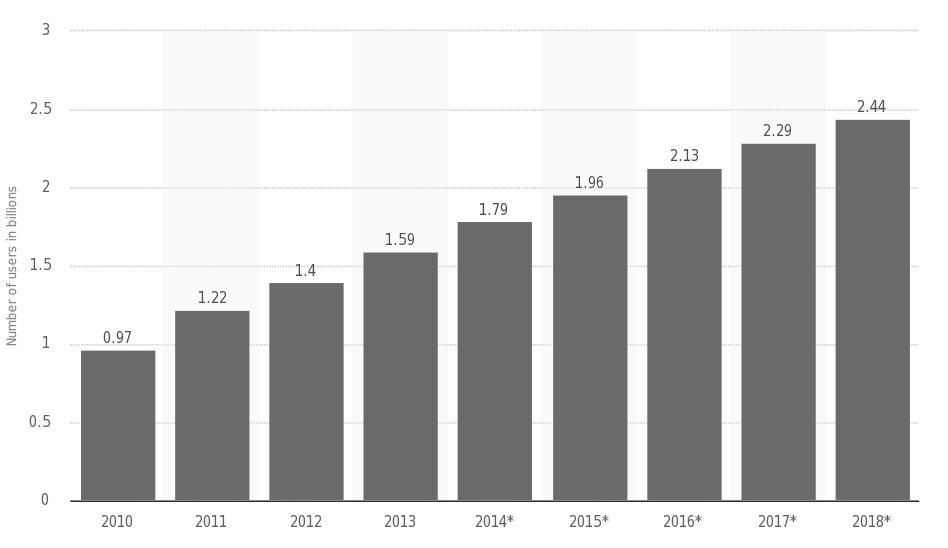
\includegraphics[width=\linewidth]{01_social_net_growth}
    \label{fig1:social_net_growth}
\end{figure}

In \autoref{fig1:social_net_growth} the number of social network users worldwide from 2010 to 2014 with projections until 2018 is represented. By 2018 the projection shows an astonishing amount of 2.44 billion users on social media networks, this is more than 30\% of the world's population. However, data generated from systems must be mined and analyzed to represent valuable information for interested parties. This master thesis aims to explore an approach called "Entity Based Sentiment Classification" to tackle this challenge.  

As shown on \autoref{fig1:social_net_growth} in the past few years, there has been an increase in the usage of social networking services such as Twitter. Twitter, as a micro-blogging system, allows users
to publish tweets of up to 140 characters in length to tell others what they are doing, what they are
thinking, or what is happening around them. Therefore, companies and media organizations are constantly looking for ways of extracting public opinions and feelings about their products and services~\cite{kouloumpis2011twitter}. The nature of the tweets (short and usually meaningful in the context of marketing) allows researchers to exploit different data mining and sentiment analysis approaches. Projects like Twitratr\footnote{\url{http:www.twitrratr.com}}, streamcrab \footnote{\url{http:www.streamcrab.com}}, and Talend\footnote{\url{http:www.talend.com}} are examples of services intending to obtain sentiment information from tweets.

\clearpage

\autoref{tab:tweets_sentiment} shows two example tweets together with their corresponding
sentiment. The first tweet expresses a positive sentiment, containing one positive noun \textit{happy} and one positive emoji :D. The sencond tweet indicates negative sentiment based on the hashtag \textit{\#sad } and emoji :(.

\begin{table}[H]
    \centering
    \caption{Example tweets with sentiment}
    \label{tab:tweets_sentiment}
    \begin{tabular}{l|l}
        \textbf{Tweet Text}                 & \textbf{Sentiment}                \\ \hline
        I am so {\color[HTML]{036400}happy} with my new iPhone {\color[HTML]{036400}:D} & {\color[HTML]{036400} Positive}   \\ \hline
        I wont make it to the party {\color[HTML]{CB0000}:(}  {\color[HTML]{CB0000}\#sad}  & {\color[HTML]{CB0000} Negative} \\ \hline
    \end{tabular}
\end{table}


In other services such as Sentiment140\footnote{\url{http:www.sentiment140.com}} and IBM AlchemyAPI \footnote{\url{http:www.alchemyapi.com}} users may insert a target entity as a search query, then the system proceeds to fetch tweets in real-time containing positive or negative sentiments towards given target entity~\cite{jiang2011target}. This task is formally named \textit{Targeted Sentiment Analysis} and can be described as the extraction of positive, negative or neutral sentiment towards an input target entity on a given text. 

Most approaches that deal with \textit{Targeted Sentiment Analysis} are based on the extraction of target-independent features. In 2010, Barbosa and Feng ~\cite{barbosa2010robust} use a machine learning based classifiers for the sentiment classification of texts. However, their classifiers actually work in a target-independent way: all the features used in the classifiers are independent of the target, so the sentiment is decided no matter what the target is. Pang and Lee in 2002 ~\cite{pang2002thumbs} performed a similar sentiment classification experiment on movie reviews, on this experiment they only consider target-independent features on the classifier. Movie reviews usually concentrate opinions expressed towards a single target entity, in this case, a specific \textit{movie}. Nevertheless, this approach does not apply for entity based sentiment classification in tweets. Tweets have a very particular structure where multiple target entities may exist in the same context, given this scenario target-independent sentiment classifiers will not yield satisfactory results. 

\autoref{tab:target_independent_sentiment} illustrates two example tweets where TiSC\footnote{Target-independent Sentiment Classification according to Jian and Liu 2011} approaches can not correctly identify the sentiment towards given target entities. The first tweet does not express any positive sentiment
to given target \textit{iPhone} but instead to a second entity \textit{Amazon}; the problem is that the user is only interested on the input entity. This would be a false positive case for TiSCs. In the second tweet, a similar case is presented where target \textit{iPhone} is misclassified as positive when it should be negative, this happens because of an undetected comparison token: \textit{better than}. 

\begin{table}[H]
    \centering
    \caption{Example of unsuccessful cases by target-independent sentiment classification }
    \label{tab:target_independent_sentiment}
    \begin{tabular}{l|l|l}
        \textbf{Tweet Text}                         & \textbf{Target}       & \textbf{Sentiment}                       \\ \hline
        My new iPhone arrives today. I <3 Amazon!   & iPhone                &  Positive \\ \hline
        The Nexus 5 is \underline{better than} the new iPhone   & iPhone                & Positive \\ \hline
    \end{tabular}
\end{table}


A correct sentiment classification for given target entities is crucial for systems such as SentiTrack\footnote{Linked Data-based Social Media Analysis for Stock Market Tracking}. SentiTrack intends to find a correlations between the opinions extracted from real-time tweets and intra-day stock price variations of a set of specific companies. Therefore, an entity based sentiment classification is required for given task. Solving this issue is the main objective of this master’s thesis. In order to achieve this goal, proposed solution combines document-based (target independent) and entity-based features with a variety of sentiment classification techniques to train a Support Vector Machine (SVM) capable of producing highly accurate results for entity-based sentiment classification tasks.

\section{Contribution}

The main contributions that this thesis aims to achieve are the following:


\begin{itemize}

\item Develop an entity based sentiment classifier with state-of-the-art techniques for Twitter data analysis that yield highly accurate results on Target-based twitter corpora.

\item The project creates a high-performance sentiment classifier that integrates seamlessly with real-time analysis environments such as SentiTrack.

\item This work aims to describe an approach to perform sentiment classification based on entities position and presence of grammatical condition clauses on a given tweet text.

\item This work leads to the comparison and evaluation of different techniques for sentiment classification; since it provides exact information from the different techniques by evaluating the performance, accuracy, precision and recall.

\end{itemize}

\section{Overview of the document}

The introduction in Chapter 1 provides a short overview of the current state of social media ans sentiment analysis, the problems present on current sentiment classification approaches and the motivation for this thesis. Additionally, describes the contributions provided by this project. Chapter 2 explains what is sentiment analysis and the current state-of-the-art sentiment classification techniques, different Named-entity-recognition approaches and a theoretical background related to the social media. Chapter 3 explores the related work in the field of sentiment analysis and entity-based sentiment classification. Chapter 4 presents the proposed/built sentiment classification approach and explains its architecture and features. The evaluation of this project is developed in Chapter 5, which consists of cross-validation and performance tests. Finally, Chapter 6 presents the conclusion and possible future works, which summarizes the master’s thesis.

 % Introduction

 
 %~\cite[p. 2]{evans2008social} -> example
 
 \chapter{Background}
 \label{sec:background}
 
 
 This chapter explains the theoretical background used for the development of an entity based sentiment classifier. The chapter is divided into three sections: \autoref{sec:socialMedia} explains the basic concepts related to the social media and the social networking service Twitter. In \autoref{sec:sentAnalysis} Sentiment Analysis is defined and different state-of-the-art sentiment classification techniques are described. Finally, \autoref{sec:ner} explores existing Named Entity Recognition approaches.
 
 \section{Social Media}
 \label{sec:socialMedia}
 
Social Media refers to a set of computer-based tools that allows people, organizations and companies to share and exchange information with community networks. Moreover, Social Media tends to change with time allowing people to create content in a dynamic way and without restrictions. Therefore, there is an unquantifiable number of communities performing all kinds of activities such as blogging, posting on forums, podcasting, generating trends on social networks and more. 

The Social Media relies on various technologies to achieve a compelling communication between users. Web structures like social networks are fundamental for the social media. These structures are mainly made of actors and messages which can be visualized as graph nodes with specific properties and unique attributes. This concept is depicted on \autoref{fig2:twitter_graph} where the interaction between the different elements of the social network Twitter is represented. In \autoref{sec:twitter}, Twitter and its elements are explained in detail.

\begin{figure}
    \centering
    \caption[Twitter graph representation]{Twitter: graph representation {~\cite{kenny2014graph}}}
    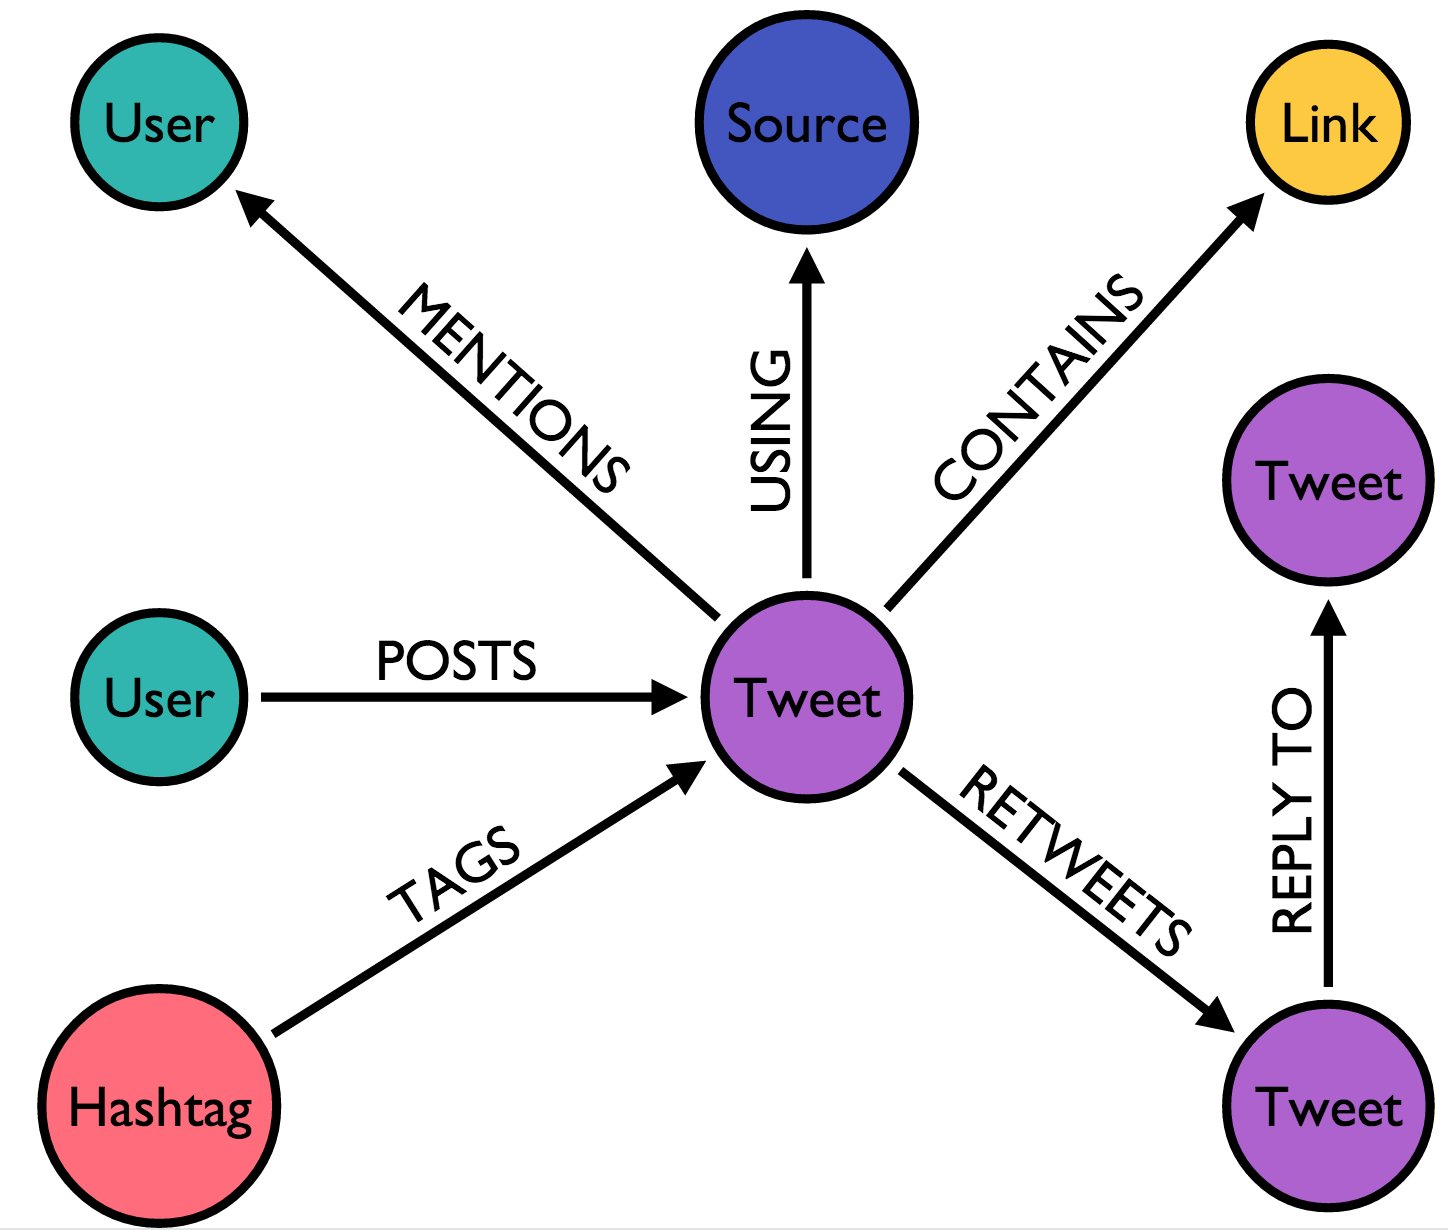
\includegraphics[width=\linewidth]{02_twitter_graph.png}
    \label{fig2:twitter_graph}
\end{figure}

\subsection{Twitter}
\label{sec:twitter}

Being one of the most popular websites in the world, Twitter has become an ever-growing corpus of information. As a social network, Twitter allows constant sharing of short messages between users; this is also called micro-blogging. Between users, they can follow the activity of each other giving updates of their messages. Currently, this network has around 320 million of active users {~\cite{statTwit2016}.

As described in \autoref{fig2:twitter_graph}, Twitter is composed of the following elements:

\begin{itemize}
\item \textbf{Tweet:} Tweets are the essence of Twitter, they are short message units (pieces of information) formed by a maximum of 140 characters. Users use tweets to share ideas, status, news or any other kind of information with their followers. In \autoref{fig3:tweet_example} a tweet example is showed where the actor: User is \textit{"Outlook"} and the message contains \textit{\#hashtags, @mentions} and \textit{URLs}. 

\pagebreak

\begin{figure}
    \centering
    \caption{A tweet example}
    
\includegraphics[width=\linewidth]{03_tweet_example.png}
    \label{fig3:tweet_example}
\end{figure} 

\item \textbf{Users:} The users are the source of information on Twitter. They have followers who are other users interested in the content being sharing.
\item \textbf{Trends:} Trends are popular topics close to the geographic location of the users. They are determined by an algorithm that combines the information about followers, accounts, and places related to them. The trends intend to help users to discover relevant topics based on their location.  
\end{itemize}

\section{Sentiment Analysis}
\label{sec:sentAnalysis} 
 
 Sentiment analysis (SA) also known as Opinion Mining can be defined as the use of computer-based methods to extract an opinion from a given text source. Liu ~\cite[p. 7]{liu2012sentiment} defines SA as: 
 \begin{displayquote}
"The field of study that 
analyzes people’s opinions, sentiments, evaluations, appraisals, attitudes, 
and emotions towards entities such as products, services, organizations, 
individuals, issues, events, topics, and 
their attributes."
\end{displayquote}
    
Opinions are essential for all human activities because they affect our decisions. Before making decisions, people usually evaluate others opinions. In the real world, businesses and organizations are always trying to know the public opinion about their
products and services and be able adapt marketing strategies~\cite[p. 10]{liu2012sentiment}. Nowadays, companies may no longer require surveys and opinion polls to gather the opinion of their customers. However, analyzing opinion sites and social networks by SA means is not an easy task. Several fields of Computer Science such as Natural Language Processing (NLP), Machine Learning (ML) and Information Retrieval (IR) are some of the research areas involved in SA. 

\subsection{Analysis Levels}

There are different levels of SA that could be applied to a given text source, these are the following~\cite[p. 11]{liu2012sentiment}:
 
\begin{itemize}

\item \textbf{Document level:} The objective of this level if SA is to classify the sentiment (positive, negative or neutral) of a whole document. Documents in this context refer to any piece of information that requires analysis. Tweets, .pdf files, forums posts, e-commerce reviews, all are considered documents for sentiment analysis porpoises. Sentiment classification of product reviews on e-commerce system are good examples of these level of analysis. Document level SA is effective on text sources that express opinion towards a single entity. When many entities are present in the document this type of analysis may not be very accurate.

\item \textbf{Sentence level:} As its name describes, sentence level analysis segments a given document into sentences, then each of these sentences is processed for classification. Similar to \textit{document-level} SA, opinions on sentences must express its sentiment towards a single entity in order to achieve high accuracy. 

\item \textbf{Entity level:} \textit{document-level} and \textit{sentence-level} analysis are not capable of finding the target of peoples’ opinion. Entity-level is a finer-grained analysis that assumes the presence of a target entity in the opinion expression. For example, the sentence \textit{"although the iPhone is not a good phone, I still love Apple as a company"} may appear to have a positive tone but is not accurate to classify it as positive. In this case, there are two different sentiments: A positive sentiment towards the entity \textit{Apple} and a negative sentiment towards entity \textit{iPhone}. Therefore, the ultimate goal of this level of analysis is to find out the sentiment expressed towards target entities. This thesis project base its’ sentiment classification approach on this level of analysis.

\end{itemize}

\subsection{Sentiment Classification}
\label{sec:sentClassification} 

Sentiment classification is one of the most studied topics in the area of sentiment analysis and natural language processing. The main goal is to classify a document as positive or negative based on the opinion expressed in it, if the document does not contain any opinion expression the classification result must be neutral. The following sections present unsupervised and supervised techniques for sentiment classification according to Bing Liu~\cite{liu2012sentiment}.

 

 
 \subsubsection{Unsupervised Techniques}
 
 Unsupervised techniques for sentiment classification are strongly based on opinion words, also known as lexical resources. Consequently, these techniques classify documents using lexicon-based methods. Every word contained in a document or input text is evaluated for polarity orientation, this orientation is defined by the presence of opinion words, which are contained in sentiment dictionaries (lexicons). Hence, if a document contains more \textit{positive} than \textit{negative} words, the sentiment classification result of the document would be \textit{positive}. The absence of polar-oriented words in a document results in a \textit{neutral} classification~\cite[p. 29]{liu2012sentiment}. 
 
 Sentiment dictionaries or opinion lexicons are the core component of any unsupervised sentiment classification method. These dictionaries are made of words or phrases with specific sentiment scores. For example, words like \textit{fantastic} and \textit{excellent} have a positive orientation in most sentiment lexicons, while other words such as \textit{terrible} and \textit{awful} are categorized as negative. Sentiment lexicons define the polarity orientation of words by numeric values, some of them assign intensity score to each word and others consider negating contexts for sentiment scores. \autoref{sec:normalization} explains more about negation contexts.
 
 There are several way of creating a sentiment lexicon; Bing Liu explains the most effective ones~\cite{liu2012sentiment}.: 
 \begin{enumerate}

\item \textbf{Manual approach:} As its name refers to, this approach requires the effort of evaluators to manually assign sentiment orientation to a set of words. This task consumes a lot of time and its better to be used in combination with other automatic methods. However, it is useful for evaluation of results of non-manual approaches ~\cite[p. 79]{liu2012sentiment}.

\item \textbf{Dictionary-based approach:} This is arguably the most effective approach for lexicons creation, it automatically generates a sentiment dictionary based on synonyms and antonyms and the grammatical relation between words. WordNet is defined as \textit{"a large English lexical database where nouns, verbs, adjectives and adverbs are grouped into sets of synonyms called synsets, each expressing a distinct concept"}~\cite{word2016}. Although, there are many dictionary-based approaches, one of the most useful ones follows two steps. First, evaluators manually annotate a set of seed words (e.g. \textit{bad}, \textit{good}) with "obvious" polarity orientation. Then, each seed word is expanded by collecting their synonyms and antonyms from a dictionary (e.g. WordNet). After that, collected words with their respective sentiment scores are appended to the original set of seed tokens. This process is repeated progressively resulting in an expanding sentiment lexicon~\cite[p. 80]{liu2012sentiment}.

\item \textbf{Corpus-based Approach:} A corpus based approach is mostly used for the generation of domain-dependent sentiment lexicons. In this context, sentiment words are extracted from specific domain corpus or adapted from an open-domain one ~\cite[p. 82]{liu2012sentiment}. This extraction task is not a simple given that some words may express different or even opposite sentiment depending on their context. As an example, lets take the word  \textit{"unpredictable"}. An \textit{unpredictable} movie plot might be considered positive but an \textit{unpredictable} work schedules would be negative for most people. The corpus-based approach uses grammatical rules to expand a set of sentiment seed words. With the use of \textit{conjunction} words (e.g \textit{and}, \textit{yet}) it is possible to infer the sentiment orientation of unclassified words. In the following sentence: \textit{"the computer is powerful and fast"} if the word \textit{powerful} is a positive oriented seed word, we can infer that \textit{fast} is also positive. Therefore, a domain specific lexicon expansion relies the presence of \textit{Conjunctions}.

\end{enumerate}

\begin{figure}
    \centering
    \caption[Penn Treebank Part-Of-Speech (POS) tags]{Penn Treebank Part-Of-Speech (POS) tags{~\cite[p. 33]{liu2012sentiment}}}
    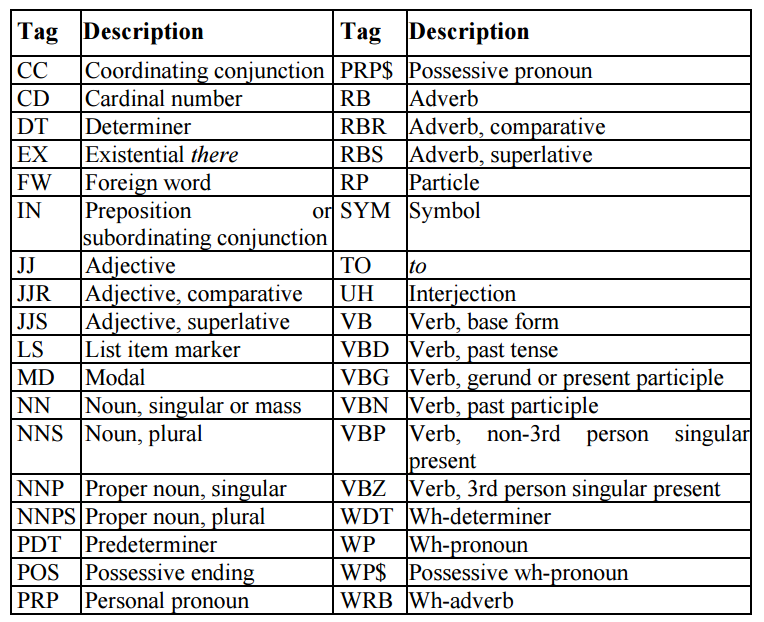
\includegraphics[width=\linewidth]{04_treebank_pos}
    \label{fig4:treebank_pos}
\end{figure}


\autoref{tab:unsupervised_example} illustrates the sentiment classification of two example tweets using a lexicon based unsupervised technique where positive and negative words are evaluated to +1 and -1 respectively. The overall score of each tweet is calculated by adding up the sentiment values of individual words.

 \subsubsection{Supervised Techniques}
 
 Supervised sentiment classification can be categorized as a natural language processing task (text classification). There are many methods to perform text classification, some of the most used classifiers are Maximum Entropy, Naive Bayes and Support Vector Machines (SVM). Before starting a sentiment classification task, the number of classes must be defined. The following are the most common approaches~\cite{liu2012sentiment}:
 
 \begin{itemize}
  \item \textbf{Two-class classifier}: Also known as polarity classification, has as an objective to classify a document as \textit{positive} or \textit{negative} which represent the two classes respectively.
  
  \item \textbf{Three-class classifier}: Similar to the two-class classifier, this one also includes subjectivity classification which means that it classifies documents as \textit{neutral} or \textit{polar} (positive or negative).
  
  \item \textbf{Multi-class classifier}: A multi-class sentiment classifier is usually based on emotional classification. Therefore, documents are classified according to emotions expressed on them (e.g. \textit{angry}, \textit{sad}, \textit{happy}, etc). 
  
\end{itemize}

\begin{table}[]
\centering
\caption{Unsupervised classification of tweets example.}
\label{tab:unsupervised_example}
\begin{tabular}{l|l}
\textbf{Tweet Content}                                                           & \textbf{Score} \\ \hline
{\color[HTML]{000000} @TylorSwift concerts are the best{\color[HTML]{036400}(+1)} :D{\color[HTML]{036400}(+1)} \#hypped{\color[HTML]{036400}(+1)}} & {\color[HTML]{036400} 3} \\ \hline
@Apple please stop selling terrible{\color[HTML]{CB0000}(-1)} music on iTunes \#mad{\color[HTML]{CB0000}(-1)}                & {\color[HTML]{CB0000}-2}                       \\ \hline
\end{tabular}
\end{table}

\pagebreak

One of the main differences between unsupervised and supervised sentiment classification methods is the training phase. Sentiment classifiers based on supervised approaches require a set of annotated documents, this annotation is usually done manually but in some cases through distant-supervision methods~\cite{go2009twitter}. Distant-supervision approach generates a training corpus by automatic means. It annotates documents based on the presence of positive or negative emojis (emoticons). The annotation accuracy of this method depends on the size of the documents, mostly used on short unit texts such as Twitter sentiment classification tasks. 

After being trained, a classifier is capable of predicting the sentiment of new input documents. The classification process requires the extraction of feature vectors from the documents; each vector contains \textit{n} numerical features. The feature sets of a classifier are essential for obtaining high accuracy. Some of the most effective features are~\cite[p. 25]{liu2012sentiment}: 

 \begin{itemize}
  \item \textbf{Terms and their frequency (bag-of-words model)}: These features are individual words (unigrams) or n-grams with associated frequency counts. N-grams are a contiguous sequence of n-tokens (words) from a given sequence of text. Besides frequency counts of the tokens, their positions might be also considered. This approach is called TF-IDF weighting scheme and is commonly used in information retrieval tasks.

    \item \textbf{Part of speech}: The part-of-speech (POS) of words in a document could be useful. For example, some research shows that adjectives are more likely to indicate sentiment than other part-of-speech words. Therefore, the number of different POS tags in a given document represents an effective feature. POS tags may also be included in other types of features such as \textit{Terms and their frequency} where unigrams are included with their respective POS tag.
    
    \item \textbf{Sentiment words and phrases}: As discussed in previews section, the presence of positive and negative words is very important for sentiment classifiers. Extracted from sentiment lexicons, the number of sentiment terms and phrases in a document represents very powerful features. 
    
    \item \textbf{Syntactic dependency}: The semantic relation between words in a document may be useful as a feature, with the usage of dependency trees is possible to find the target of a sentiment expression. However, the creation of these trees usually has a negative impact in performance times. 
    
    \item \textbf{Sentiment shifters}: These are expressions that are used to change the sentiment orientations, e.g., from positive to negative or vice versa~\cite[p. 26]{liu2012sentiment}. The most important type of sentiment shifters is negation contexts. When a negation word (e.g. \textit{not, no, never}) is present in a sentence, the sentiment score of subsequent words is inverted. For example, the sentence \textit{"the iPhone is not a good phone"} has the word \textit{good} in a negated context which translates to a negative sentiment classification of the sentence.
    
    \end{itemize}

    \begin{table}[]

    \end{table}
   

    \autoref{tab5:features_example} illustrates two example tweets with their respective vector features, these features are composed by Bag of Words model, part-of-speech tags and sentiment features. Let us explain one by one: 
    
    \begin{itemize}
        \item \textit{bag-of-words}: To reduce the sparsity of the vectors, one of the most used prepossessing steps for extracting features is the removal of stop words, which in these cases are: \textit{you, the, my, me, are}. Twitter mentions and URLs are also removed or replaced with placeholders. The resulting vectors are: 
        \begin{itemize}
            \item (1) {(@mention,1)(best,1)(<3,1)(\#happy,1)} 
            \item (2) {(bf,1)(hates,1)(:(,1)(depressed,1)}
        \end{itemize}
        Each tweet is represented on the vector space which is the union of both sets.
        
        \item \textit{part-of-speech}: This feature is composed by the count of: \textit{verbs, adjectives, nouns, adverbs}. Other POS tags could be added but these are the most relevant for sentiment classification tasks.
        
        \item \textit{sentiment}: The first tweet contains three positive tokens while the second one has three negative. As a result, the sentiment features are: (1)[3,0] \& (2)[0,3].
        
    \end{itemize}
    
    \pagebreak
    
    \subsection{SentiTrack}
    \label{sec:sentitrack}
    
    SentiTrack is a system that performs sentiment analysis of tweets in real-time using Semantic Web technologies to track stock market behaviors of a certain set of companies. In order to determine the public opinion towards a company, SentiTrack uses the Twitter API to pull tweets related to that company and process them through a sentiment analysis pipeline~\cite{danklinked}. An illustration of SentiTrack's process workflow is shown in \autoref{fig14:sentitrack_workflow}. 
    
    SentiTrack processing workflow is divided into the following three stages:
    
    \begin{enumerate}
        \item \textbf{Context Expansion}: In this stage, SentiTrack starts by selecting the set of entity companies to analyze. Then, using DBPedia and SPARQL queries a retrieval of secondary entities related to those chosen companies is performed. The secondary entities in this context are \textit{persons} and \textit{products}, e.g. \textit{Company: Microsoft, Person: Bill Gates, Product: Windows}. 
        
        \item \textbf{Stream Processing}: The set of entities obtained in previews stage are used to fed the Twitter Streaming API in order to fetch related public tweets in real-time. Then, tweets are processed for recognition and annotation of entities using DBPedia Spotlight. Moreover, those tweets with annotated entities are analyzed using a lexicon-based entity-centric sentiment classifier. The classification step intends to provide a positive, negative or neutral result based on the opinions expressed towards each of the identified entities in the tweet. Entity-centric sentiment classification approach used by SentiTrack is vary simple and not accurate enough. Therefore, an improved entity-based sentiment classifier is required for SentiTrack project.
        
        \item \textbf{Periodic Sentiment Approximation}: This stage is about analysis of the sentiment data obtained in previews steps. It creates a periodic sentiment projection in real-time about the opinions expressed in Twitter towards a target company. Additionally, a secondary system fetches real-time stock market values about the target company, this is necessary to perform a correlation evaluation with sentiment data obtained and stock values variations. 
        
    \end{enumerate}
    
    One of the contributions of this master's thesis is to integrate a more accurate sentiment classifier in SentiTrack.  
    
    \begin{figure}[H]
    \centering
    \caption[SentiTrack Workflow]{SentiTrack Workflow{~\cite{danklinked}}}
    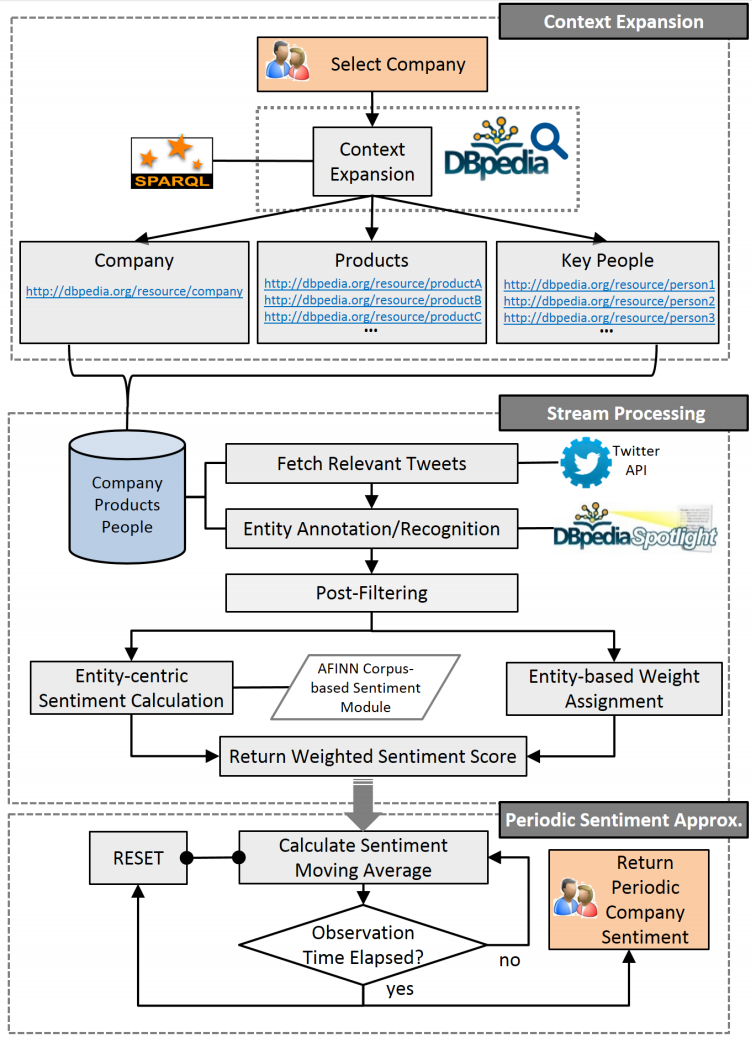
\includegraphics[width=\linewidth]{14_sentitrack_workflow}
    \label{fig14:sentitrack_workflow}
    \end{figure}
    
    \section{Named Entity Recognition}
    \label{sec:ner}
    
    Named Entity Recognition (NER) also known as named entity extraction or entity identification, is an information extraction task used mostly for natural language processing. The task consists on the extraction of structured information from unstructured text, for instance: social media networks, micro-blogging sites and e-commerce systems are constantly generating unstructured data that could be processed into valuable information for interested parties. Therefore, NER intendeds to identify elements of given input text and classify it according to a set of categories, e.g. names of persons, locations, organizations, products, values, etc ~\cite[p. 1]{nadeau2007survey}. 
    
    The most effective approaches for NER use machine learning (ML) methods to extract features of Named Entity (NE) examples classified as positive or negative, finally, these examples will form a large collection of annotated documents (training corpus).   
    
    There are three main ML techniques to perform entity identification  ~\cite[p. 4]{nadeau2007survey}:
    
    \begin{enumerate}
        \item \textit{Supervised learning}: Some of these techniques are Maximum Entropy, Decision Trees, Support Vector Machines, Conditional Random Fields and according to Nadeau ~\cite[p. 4]{nadeau2007survey}:
        \begin{displayquote}
            "A baseline Supervised learning method that is often proposed consists of tagging words of a test corpus when they are annotated as entities in the training corpus. The performance of the baseline system depends on the vocabulary transfer, which is the proportion of words, without repetitions, appearing in both training and testing corpus."
        \end{displayquote}
        Which means that NER is highly dependent on the quality of the training corpus, this will determine how accurate the classifier is.  
        
        \item \textit{Semi-supervised learning}: Semi-supervised learning (SSL) consist of a limited degree of supervision. Therefore, this technique only requires a set of seed words to start a learning process. For example, the system starts with a set of seed words related to a specific topic such as "technology". Then, the system identifies contextual clues of given words to classify new unknown terms. The accuracy this approach can achieve is not as high as fully supervised learning techniques but is effective for identification of entities related to unpopular topics where good training corpus are difficult to find. 
            
        \item \textit{Unsupervised learning}: This is a NER technique that usually depends on lexical resources (e.g., WordNet) to identify entities in a document. The types of entities are extracted from given Lexicons, therefore, the quality and number of lexical resources will define the success of this technique.
        
    \end{enumerate}
    
    
  

 
 
 
 
 

   
 
 
 
 
 
 
  % Background


\chapter{Related Work}
\label{sec:related_work}


This chapter presents a variety of projects and scientific work related to sentiment analysis and the usage of entity based approaches for sentiment classification. The constant publication of opinionated data in social media networks provides an ever-growing source of valuable information for interested companies. Therefore, Sentiment Analysis has become a very popular research field in the scientific community. Pang and Lee ~\cite{pang2008opinion} in 2008 presented a survey that covers techniques and approaches for polarity sentiment classification and subjectivity identification. Moreover, in 2012 Bing Liu ~\cite{liu2012sentiment} published one of the most cited books related to sentiment analysis, where he provides a very complete survey of most relevant research topics related to opinion mining. 

Based on aforementioned literature and additional related works, the next section discusses a variety of sentiment analysis projects and the different approaches used in them. Finally, this chapter presents a few research works associated with entity-based sentiment classification and compares these techniques with the methods utilized and developed in this master's thesis.

\section{Sentiment Analysis}


The applications of Sentiment analysis are many, some of them include the classification of forum posts, blogs, news, product reviews and social network content. Therefore, because this thesis project is based on social media analysis, specifically Twitter data. The related work presented in this section is mainly focused on document-level sentiment analysis of tweets.

\pagebreak

The term of sentiment analysis was first introduced by Nasukawa and Yi in 2003 ~\cite{nasukawa2003sentiment}, in their work they extracted sentiments associated with polarities of positive or negative for specific subjects using semantic analysis with a syntactic parsing method. However, research about opinions and sentiments expressed in text appeared in 2001 where Das et al.~\cite{das2001yahoo} and Tong~\cite{tong2001operational} published their work about the analysis of market sentiment. 

It was not until 2009 where Bhayani et al.~\cite{go2009twitter} presented the first relevant research related to the usage of Twitter data for sentiment analysis. Bhayani et al. used a novel approach for automatic polar-classification of tweets where messages are classified as either positive or negative. Based on distant supervision and machine learning algorithms, Bhayani et al. generated a training corpus evaluating the presence of positive or negative emoticons such as ":D" or ":(" in each tweet. With this method, they managed to achieve an accuracy above 80\% for a polarity classification task.

In 2010 Pak and Paroubek~\cite{pak2010twitter} built a sentiment classifier that is able to determine positive, negative and neutral sentiments of English tweets. Using a distant supervision approach similar to Bhayani et al.~\cite{go2009twitter} for the generation of a training corpus, they implemented a multinomial Naive Bayes classifier extracting POS-tags and unigrams as binary features. In their results they showed higher precision by using a term presence rather than its frequency. Also, an increased accuracy was obtained by the usage of unigrams instead of bi-grams or three-grams. On the other hand, Barbosa and Feng in same year~\cite{barbosa2010robust} presented a 2-step sentiment analysis classification method which first classifies tweets as subjective and objective (neutral and polar), followed by a polarity classification of subjective tweets as positive or negative. Based on support vector machines, this 2-step approach proved an increased accuracy in comparison with single step classifiers. 

In 2011 Kouloumpis et al.~\cite{kouloumpis2011twitter} explored the utility of linguistic features
for the identification of sentiment in Twitter messages. This paper presents an extended distant supervision approach for generation of training data, the methods used consist on the inclusion of Twitter hashtags such as \textit{"\#bestfeeling, \#epicfail, \#news, etc."} to enhance the training data quality and include a third class to the classifier (neutral). Additionally, Kouloumpis et al. implemented a 3-step prepossessing method composed by the following steps: (1)tokenization, (2)normalization, (3)part-of-speech tagging. According to Kouloumpis et al.'s results this prepossessing stage improves the quality of the extracted features. In contrast to Kouloumpis et al., the methods used by Paltoglou and Thelwall~\cite{paltoglou2012twitter} in 2012 explored an unsupervised lexicon-based approach that predicts the level of emotional intensity contained in tweets. According to Paltoglou and Thelwall, this approach may be used for subjectivity identification and sentiment classification tasks, obtaining results comparable to state-of-the-art machine learning based methods.


In 2013 Saif et al.~\cite{MohammadKZ2013} developed a state-of-the-art support vector machine (SVM) classifier which obtained the best results in SemEval 2013 Twitter analysis task. SemEval (Semantic Evaluation) is an international competition for evaluations of computational semantic analysis systems. Many scientist and students from all around the world participated in this event, but Saif et al.'s sentiment classification approach excelled in its category. The classifier uses a large set of features to train a SVM, features such as n-grams, POS-Tags, hashtags, lexicons, emoticons, elongated words are just a part of the full set. However, the addition of negation context handling was one of the determinant factors to outperform the other competitors. Finally, the methods presented in this master's thesis for document-level features extraction are highly influenced by Saif et al.'s work.

\section{Entity Based Sentiment Analysis}

Currently, there are not many research works related to entity based sentiment analysis in Twitter. Therefore, this section intends to discuss the most relevant publications that explore the idea of an entity-centric sentiment classifier. Starting with Ding et al.~\cite{ding2008holistic}, in 2008 they presented a holistic lexicon-based approach to perform topic-based opinion mining. In their work, they determined the sentiment orientations (positive, negative or neutral) of opinions expressed in product features in reviews. With the usage of unsupervised lexicon-based techniques, Ding et al. defined a set of linguistic rules to extract opinion phrases expressed towards specific products in a given review text. Although Ding et al.'s approach achieved high accuracy for topic-based sentiment analysis on product reviews, this method may not perform just as well with noisy text such as tweets. Khoo et al.~\cite{thet2010aspect} in 2010 implemented an aspect-based sentiment classifier which was capable of extracting both sentiment orientation and sentiment strength of movie reviews. He considered the sentiment expressed towards different aspects of these movies. These aspects can be seen as sentiment targets, using sentence oriented linguistic clauses, Khoo et al. managed to obtain highly precise sentiment scores for movie aspects. However, one of the drawbacks of Khoo et al.'s solution is the absence of a neutral class on their approach. 



The most relevant scientific work related to this master's thesis was developed by Jiang et al.~\cite{jiang2011target} in 2011. They focused on target-dependent Twitter sentiment
classification which means that given an input query, they classify the sentiment orientation of the tweets as positive, negative or neutral based on the presence of positive, negative or neutral sentiments towards that query. In Jiang et al.'s approach they implemented a two-step SVM classifier incorporating
target-dependent and target-independent features. Additionally, they included related tweets (mentions and replies of each tweet) in the analysis. According to their experimental results, the two-steps methodology greatly improves the accuracy of entity-based sentiment classifiers. Nevertheless, because of the complexity of the methods and the necessity of analyzing related tweets in each document, the performance time is compromised and not suitable for real-time systems.

To conclude this chapter is important to clarify that this master's thesis is highly influenced by aforementioned research works. However, the specific combination of methods and techniques used in this project are not documented in any other related publication.   

 % Smart Semantic Service for CSP,India


\chapter{Approach}
\label{sec:approach}

This chapter gives a comprehensive description of the development of an Entity-based Sentiment Classifier for social media analysis, which is the ultimate result of this thesis. This approach relies on natural language processing (NLP) methods and machine learning (ML) tools to achieve a highly accurate sentiment classification. 

The following section presents the architecture and process pipeline of the entity-based sentiment classifier. Moreover, following sections provide an in depth description of the architecture's components.

\section{Architecture}

The architecture composition of the entity-based classifier is represented as a pipeline of processes. Each process is essential for the correct operation of the classifier, which is the following: 

\begin{enumerate}
\itemsep0em 

\item \textbf{Entity identification}

\item \textbf{Tokenization}

\item \textbf{Normalization}

\item \textbf{POS-Tagging}

\item \textbf{Feature Vector Generation}
\subitem - Document-based features
\subitem - Entity-based features

\item \textbf{Support Vector Machine}

\end{enumerate}

\begin{figure}
    \centering
    \caption{Processing pipeline and architecture}
    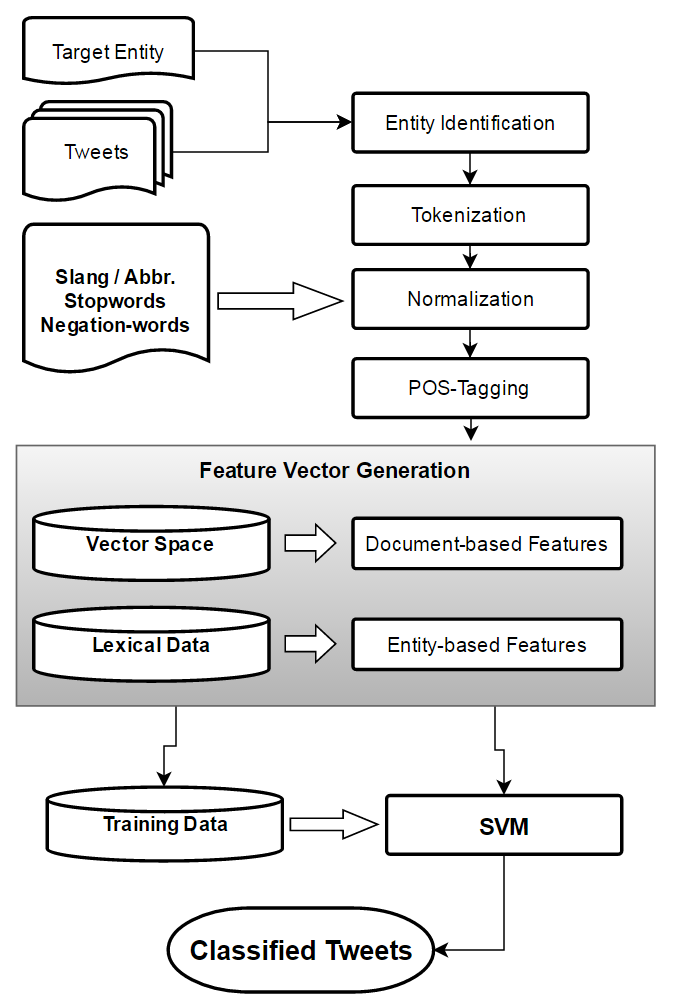
\includegraphics[width=\linewidth]{05_architecture}
    \label{fig5:architecture}
\end{figure}

\autoref{fig5:architecture} illustrates aforementioned components and processes. The pipeline starts with two input elements provided by the user or system which the classifier is integrated to. The required input data are the following:

\begin{itemize}
\itemsep0em 

\item \textbf{Tweet:} are microblogging-posts shared on the social media network Twitter. Tweets have a restriction of 140 characters and may contain URLs, mentions, hashtags or multimedia content. The classifier proposed in this thesis should be able to process every word or phrase contained in tweets in order to yield an accurate sentiment classification. For this task, specialized natural language processing methods are necessary.

\item \textbf{Target Entity:} The target entity refers to a query term (usually a company, product or person) which the classifier takes as an input in order to find the opinion expressed towards it. Therefore, given target entity must be present in the tweet. 

\end{itemize}

\begin{figure}[H]
    \centering
    \caption{Simplified entity-based sentiment classifier workflow}
    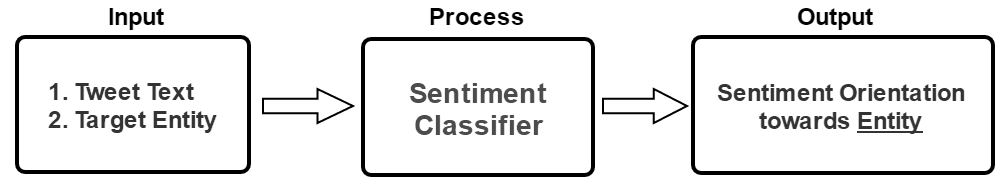
\includegraphics[width=\linewidth]{06_input_output}
    \label{fig6:input_output}
\end{figure}

\autoref{fig6:input_output} shows a simplified workflow of the entity-based sentiment classifier developed in this thesis. Notice that the input of the classifier is a 2-tuple (two elements list) composed by a tweet and a target entity. The output produced by the classifier is a three-class sentiment classification (positive, negative or neutral) which represents the opinion expressed in the tweet towards given target entity. Furthermore, continuing with the explanation of \autoref{fig5:architecture}, the first processing step in proposed system is called Entity Identification which will determine the presence of other entities (besides the target one) in the tweets. Then, the Tokenization step proceeds to remove unnecessary tokens (terms or words) or replace them with predefined placeholders. The workflow continues with a normalization process which is responsible for most of the linguistic processing in input tweets. After obtaining a normalized data, a POS-Tagger assigns part-of-speech labels to each token and sends them to the Feature Vector Generator. The Feature Vector Generator proceeds to extract document and entity level feature vectors to finally feed the support vector machine. The following sections will describe how each of these processes work.   

\pagebreak

\section{Entity Identification}

Entity identification, also known as Named-entity recognition (NER), is an information retrieval task that intends to label tokens of a given text into pre-defined categories such as companies, persons, locations, etc. The proposed approach requires the identification of entities in tweets to isolate contextual sentiments expressed towards the target entity. Therefore, opinions expressed towards non-target entities are not considered for sentiment classification. In following sections the entity contextual separation process is explained. 

\begin{figure}[H]
    \centering
    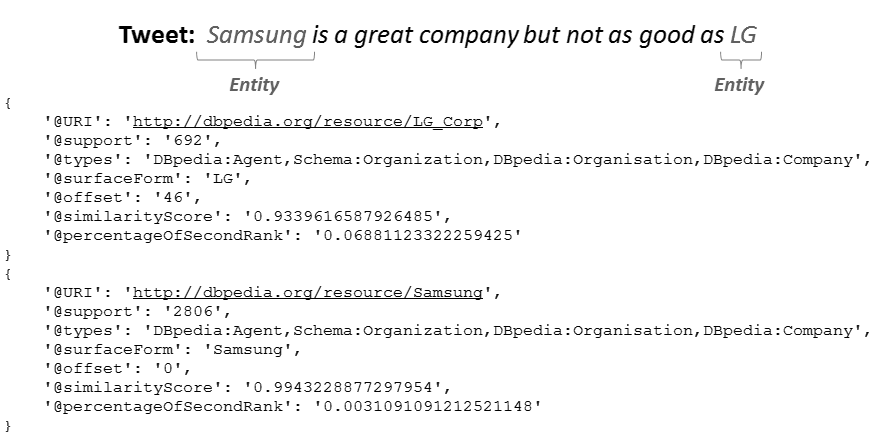
\includegraphics[width=\linewidth]{07_dbpedia_spotlight}
    \caption{DBPedia Spotlight annotation example}
    \label{fig7:dbpedia_spotlight}
\end{figure}

Proposed sentiment classification approach uses DBpedia Spotlight service in order to carry the entity identification task. This service annotates DBpedia\footnote{\url{http:wiki.dbpedia.org}} resources contained in the tweets, generating a list of contained entities. \autoref{fig7:dbpedia_spotlight} presents an example text annotated by Dbpedia Spotlight service which in this case provides meta-data about two identified DBpedia resources: \textit{Samsung} and \textit{LG}. Although the service returns information about entities such as \textit{type} and \textit{DBPedia URI}, proposed classifier only considers the identification of existing entities in given text ignoring the rest of the information. Further usage of DBpedia Spotlight service might be explored for future works and enhancements. Finally, a list of extracted entities is forwarded to the Tokenizer module which is explained in next section. 

\pagebreak

\section{Tokenization}

The Tokenization process is responsible for splitting input tweet text (string) into tokens (word or terms) and organize those tokens into their respective sentences. The Tokenizer (module in charge of this process) uses natural language processing methods and logistic rules such as regular expressions to trim the text. 

\begin{figure}[H]
    \centering
    \caption{Tokenization workflow}
    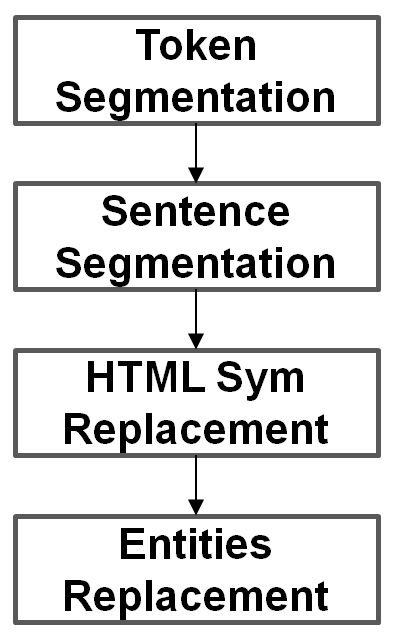
\includegraphics[width=6cm,height=9cm,keepaspectratio]{08_tokenization}
    \label{fig8:tokenization}
\end{figure}

In \autoref{fig8:tokenization} the Tokenization process workflow is represented. Starting with the \textit{token segmentation}, words contained in tweets are separated to each other based in the presence of white spaces. Then, a regular expressions algorithm checks each of those tokens for sentence stop punctuations such as exclamation points, question marks and full stops. This sentence segmentation step is necessary for the entity-based feature vector generation process since the sentiment relevance of sentences is associated with the presence of entity tokens. Finally, HTML symbols (e.g. \&amp, \&quot, etc) are replaced by their substituted values (some emoticons are made by this symbols) followed by the replacement of identified entities with respective placeholder. The replacement process of entities reduces the sparsity of future generation of vector space model. \autoref{tab:tokenizer_example} shows an example of a tokenized tweet where tokens are arranged into sentences and entities are replaced by their respective placeholders (\textit{TargetEntity and OtherEntity}).

\begin{table}[H]
\centering
\caption{Tokenized tweet example}
\label{tab:tokenizer_example}
\begin{tabular}{c|l}
{\color[HTML]{000000} \textbf{\begin{tabular}[c]{@{}c@{}}Target\\ Entity\end{tabular}}} & {\color[HTML]{000000} (1) Google}                                                                                                                    \\ \hline
\textbf{\begin{tabular}[c]{@{}c@{}}Other\\ Entities\end{tabular}}                       & (1) Nexus                                                                                                                                            \\ \hline
{\color[HTML]{000000} \textbf{Tweet}}                                                   & {\color[HTML]{000000} Thanks google!! Just got my new Nexus \&lt;3}                                                                             \\ \hline
{\color[HTML]{000000} \textbf{Result Tokens}}                                            & {\color[HTML]{000000} \begin{tabular}[c]{@{}l@{}}(1) \{Thanks, TargetEntity!!\}\\ (2) \{Just, got, my, new, OtherEntity, \textless3\}\end{tabular}}
\end{tabular}
\end{table}


\section{Normalization}
 \label{sec:normalization}

Executed by a preprocessor module, the normalization step does most of the linguistic processing required for generation of feature vectors. Normalization of data involves the correction, removal and replacement of tokens yield by the tokenization process.  While some Twitter features like \textit{@mentions} and \textit{URLs} are weightless in a sentiment context, \textit{\#hashtags} actually might contain sentiment value which is necessary for a final classification. The Normalization process is composed of five processing steps, these are represented in \autoref{fig9:normalization}. 

\begin{figure}[H]
    \centering
    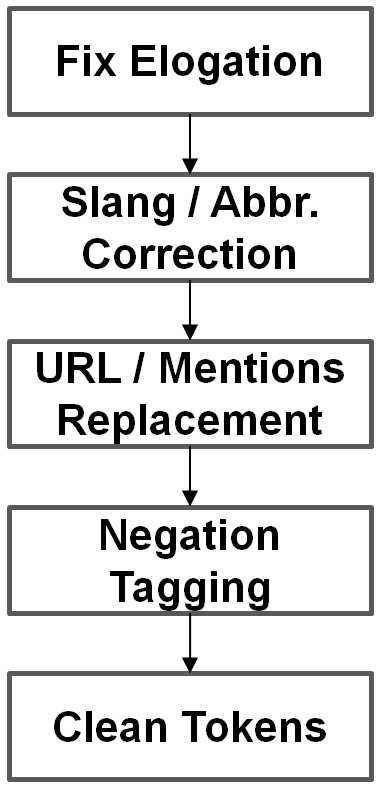
\includegraphics[width=7cm,height=10cm,keepaspectratio]{09_normalization}
    \caption{Normalization workflow}
    \label{fig9:normalization}
\end{figure}

\begin{itemize}
\itemsep0em 

\item \textbf{Fix Elongation}: tokens that contain more than two repeated letters are fixed, leaving only two of these letter. For example, the word: \textit{"loooove!"} would be replaced by \textit{"loove!"}. This process contributes with the effectiveness of the classifier because despite the fact that resulting fixed words might not necessary be the correct ones (originals), most lexicons consider two-letter elongated versions of terms.   

\item \textbf{Slang / Abbr. Correction}: presence of slang words and abbreviations are very common in microblogging sites such a Twitter. Therefore, to enhance the effectiveness of the lexicon features, these tokens are substituted by their correct forms. For example, the slang word \textit{"w8"} is replaced by \textit{"wait"} and \textit{"u"} replaced by \textit{"you"}. 

\item \textbf{URLs / Mentions Replacement:} in some cases URLs or user names (@mentions) are relevant for opinion extraction. The values by them self are ignored, but the fact that there are references to URLs and users might be useful. Hence, URLs and mentions are replaced by the placeholders \textit{"someURL"} and \textit{"someUser"} respectively.

\item \textbf{Negation Tagging}: negation words such as \textit{"not"} or \textit{"never"} can modify the sentiment orientation of a sentence. e.g. "I love you" is an obvious positive sentence, but "I do not love you" is considered negative. Therefore, to deal with this situation, a negation tagging "\_NEG" must be appended to tokens located between a negation word and the end of sentence. The sentiment of negated tokens will be shifted in the features generation stage of this classifier.  

\item \textbf{Clean Tokens}: As the final step in the normalization process, a removal of unnecessary tokens must be done. Stopwords like \textit{"you", "my" or "the"} do not represent any sentiment value, consequently, those are removed. Also, tokens with no letters (excluding emoticons) are ignored for further processing. 

\end{itemize}

\begin{table}[H]
\centering
\caption{Normalization example}
\label{tab:normalization_example}
\begin{tabular}{l|l}
\multicolumn{1}{c|}{{\color[HTML]{000000} \textbf{Tokens}}}                                                                      & \multicolumn{1}{c}{{\color[HTML]{000000} \textbf{Normalization Result}}}                                                                  \\ \hline
{\color[HTML]{000000} \begin{tabular}[c]{@{}l@{}}(1)\{not, their, best, !\}\\ (2)\{ http://t.co, @Muse, \#LiveMuse\}\end{tabular}} & {\color[HTML]{000000} \begin{tabular}[c]{@{}l@{}}(1)\{not, their\_NEG, best\_NEG, !\}\\ (2)\{ someURL, someUser, \#LiveMuse\}\end{tabular}}
\end{tabular}
\end{table}

\autoref{tab:normalization_example} presents an example of how the normalization process works, in this case two sentences are normalized. The first one shows the negation tagging of tokens \textit{"their" and "best!"} because they are positioned after the negation word \textit{"not"}. On the second sentence, an example of token replacements is shown.

\section{POS Tagging}

POS tagging consists on labeling normalized tweet tokens with their respective part-of-speech (POS) values. There are many POS tagging technologies but only a few of them are design to perform Twitter-specialized POS analysis. The solution proposed in this master's thesis uses Twitter ARK POS Tagger which is a java-based part-of-speech tagger for English data and it is tailored made for Twitter posts. ARK POS Tagger was developed by a group of researchers from Carnegie Mellon University\footnote{\url{http://www.cmu.edu/}}, they manually annotated 1,827 tweets with POS tags and developed a specialized POS tagset for tweets. ARK POS Tagger reports nearing 90\% accuracy~\cite{gimpel2011part} making it one of the most effective solutions available.  

\autoref{fig10:pos_table} shows the ARK POS tagset with examples for each POS tag. The most relevant POS tags for sentiment classification are adjectives \textit{(tag:A)} and nouns \textit{(tag:N)} which usually express some degree of sentiment. For this reason, sentiment lexicons like \textit{SentiWordNet} and \textit{AFINN} are mostly composed by nouns and adjectives. However, hashtags \textit{(tag:\#)} in tweets may also contribute significantly with the extraction of sentiment expressions. For example, the hashtag \textit{\#BeautifulDay} clearly has a positive connotation. 

\begin{table}[H]
\centering
\caption{ARK POS Tagging example over normalized tokens}
\label{tab:pos_tagging_example}
\begin{tabular}{l|l}
\multicolumn{1}{c|}{{\color[HTML]{000000} \textbf{Normalized Tokens}}}                                                                      & \multicolumn{1}{c}{{\color[HTML]{000000} \textbf{POS Tagging}}}                                                                                      \\ \hline
{\color[HTML]{000000} \begin{tabular}[c]{@{}l@{}}(1)\{not, their\_NEG, best\_NEG\}\\ (2)\{ someURL, someUser, \#Live\}\end{tabular}} & {\color[HTML]{000000} \begin{tabular}[c]{@{}l@{}}\{R/not, O/their\_NEG, A/best\_NEG\}\\ \{ someURL, someUser, \#/\#Live\}\end{tabular}}
\end{tabular}
\end{table}

\autoref{tab:pos_tagging_example} shows how the POS tagging process works. In this example, the normalized tokens \textit{not, their\_NEG, best\_NEG and \#Live} are replaced by \textit{R/not, O/their\_NEG, A/best\_NEG and \#/\#Live} respectively. The symbol "/" is appended at the beginning of each token, even if those tokens are already tagged as negated (\_NEG). Additionally, tokens already identified on previews steps are ignored by the POS tagger. e.g. "@mentions", "URLs" and "punctuation symbols". This is the final processing step before starting the feature vector generation. Following sections will explain how these tokens are transformed into vectors that will represent  key component of proposed entity-based sentiment classifier. 

\begin{figure}[H]
    \centering
    \caption[ARK POS Tagset table with examples]{ARK POS Tagset table with examples ~\cite{gimpel2011part}}
    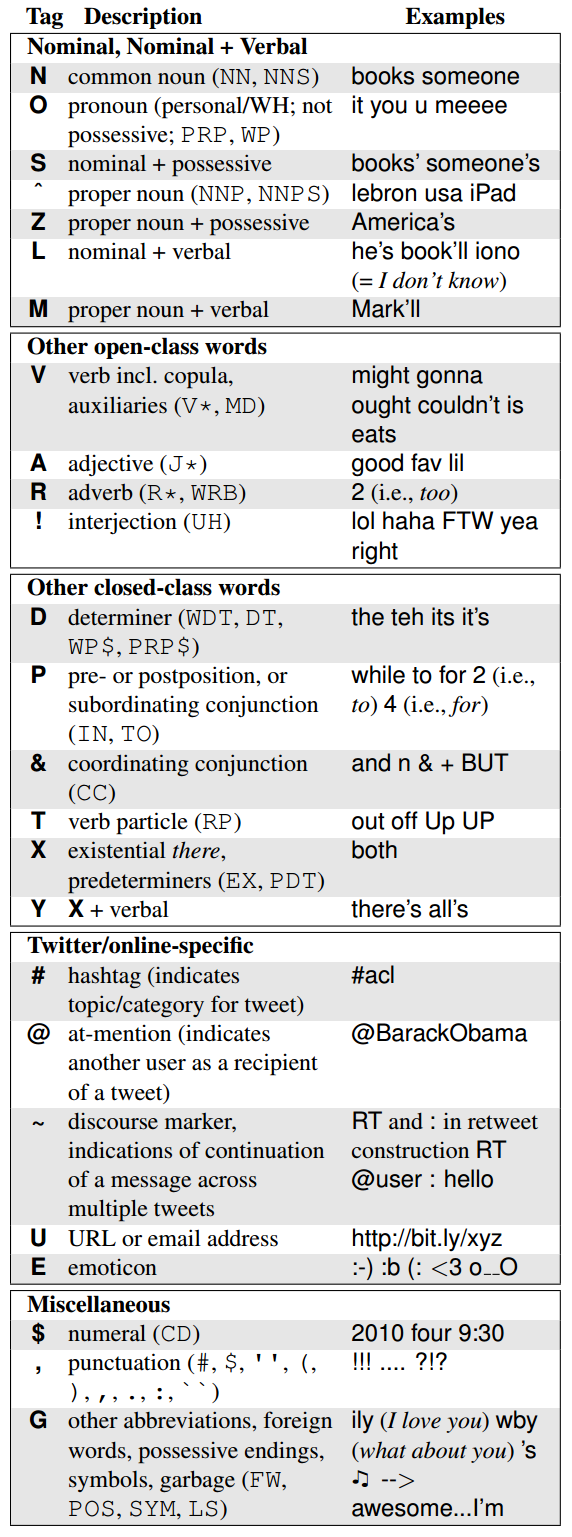
\includegraphics[width=15cm,height=23cm,keepaspectratio]{10_pos_table}
    \label{fig10:pos_table}
\end{figure}

\section{Feature Vector Generation}

The feature vector generation process is arguably the most important component in any sentiment classifier. A Support Vector Machine (SVM) based classifier like the one presented and implemented for this master's thesis, depends highly on the quality of features extracted from the raw data (tweets in this case). Therefore, in order to achieve a highly accurate classification, the production of feature vectors most be done with precision. The feature generation module is responsible for the extraction of numerical values from the already normalized and tagged tokens, the way these values are generated depends on the type of features required. Hence, this section explores two types of features: document-based and entity-based features. The sentiment classifier developed in this master's thesis uses both types of feature extraction, classifying tweets not only on a document-level like most sentiment classifiers but also on an entity-level which is the final goal of this project.   

\subsection{Document-based features generation}

Document-based features are those extracted from document-level data. This means that every single normalized-tagged token obtained from the input tweets is relevant and considered for the generation of vectors. As a result, each tweet is represented as a feature vector made up of the following set of features: binary bag-of-words (unigrams), POS tags, linguistic features.

\subsubsection{Binary bag-of-words}

Bag-of-words approach is used in natural language processing to represent training data (documents) as a set of word. This set of words is called vector space and will be made of every token existing in the training data. Then, new documents to be classified must be evaluated with aforementioned vector space to generate a vector representation of this new entry. The n-gram approach is a common way of categorizing words from documents and validate their presence in the vector space. In this master's thesis approach, unigrams were used to generate a vector space of the training data (tweets). There are many ways of representing unigrams in feature vectors but the binary approach was the selected method to be used in this project. Binary approach provides its simplicity and performance speed without scarifying quality. Binary bag-of-words also known as boolean term frequency, consists on representing terms contained in documents as 1s or 0s, where 1 means that the term is present and 0 thath it is absent. \autoref{tab:binary_bagofwords} shows an example of how a generated binary bag-of-words based on unigrams looks like.

\begin{table}[H]
\centering
\caption{Binary bag-of-words representation of a tweet}
\label{tab:binary_bagofwords}
\begin{tabular}{l|l}
\multicolumn{1}{c|}{{\color[HTML]{000000} \textbf{Tweets}}} & \multicolumn{1}{c}{{\color[HTML]{000000} \textbf{Binary Bag-of-words}}} \\ \hline
{\color[HTML]{000000} happy birthday friend! :)}            & {\color[HTML]{000000} \{1,1,1,1,0,0,0\}}                                \\ \hline
always be happy ;)                                          & \{1,0,0,0,1,1,1\}                                                      
\end{tabular}
\end{table}

\subsubsection{POS Tags}

The feature vector generated from part-of-speech (POS) Tags, consists on the number of \textit{verbs, adverbs, adjectives and nouns} contained in tweets. Inspired by Saif et al.~\cite{MohammadKZ2013}, these four POS tags are proved to be the most relevant for sentiment classification. The addition of more POS tags to the feature generation process might have a negative impact on the classification accuracy. In \autoref{tab:pos_vector} an example of POS tag features is shown, the order of POS tags for the creation of vectors is the following:  \textit{(1)noun -> (2)adjective -> (3)adverb -> (4)verb}

\begin{table}[H]
\centering
\caption{POS Tag feature vector example}
\label{tab:pos_vector}
\begin{tabular}{l|l}
\multicolumn{1}{c|}{{\color[HTML]{000000} \textbf{Tweets}}} & \multicolumn{1}{c}{{\color[HTML]{000000} \textbf{POS Tags}}} \\ \hline
{\color[HTML]{000000} happy birthday friend! :)}            & {\color[HTML]{000000} \{2,1,0,0\}}                           \\ \hline
always be happy ;)                                          & \{0,1,1,1\}                                                 
\end{tabular}
\end{table}

\subsubsection{Linguistic features}

Linguistic features are a set of elements extracted from tweets and represented as count numbers on feature vectors.  The Linguistic features consists of the following eight
elements:

\begin{enumerate}
\itemsep0em 

\item \textbf{all-caps}: the number of words with all characters in upper case.

\item \textbf{hashtags}: the number of hashtags present in the tweet.

\item \textbf{elongated words}: the number of elongated words. e.g. \textit{loooove!}

\item \textbf{negation context}: the number of negation contexts.

\item \textbf{punctuation}: count of contiguous sequences of question marks, exclamation marks, and both exclamation and question marks. e.g. \textit{!!!, ???, !!??}

\end{enumerate}

\subsection{Entity-based features generation}
\label{sec:feature_generation}

Entity-based features unlike document-based, are extracted from entity-level data. Entity-level data can be described as the context information of a target entity. The idea is to separate the contextual sentiment of every existing entity in a document (tweet in this case), then generate sentiment features only for the target entity ignoring non-target ones. Therefore, this subsection explains which entity-base features were used for the development of proposed entity-based classifier. 

\begin{figure}[H]
    \centering
    \caption{Entity-based features generation workflow}
    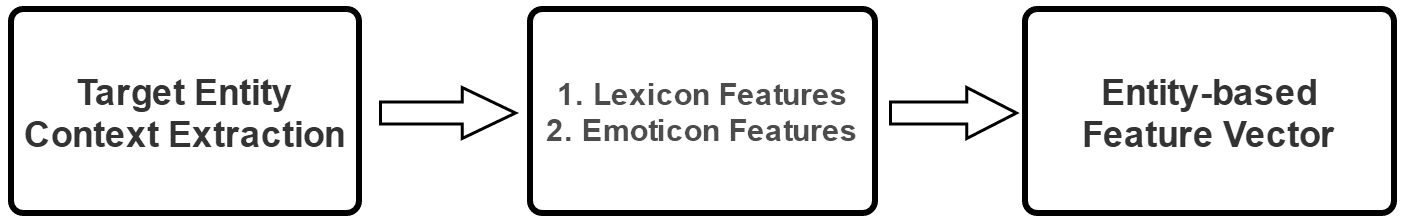
\includegraphics[width=\linewidth]{11_entity_based_features}
    \label{fig11:entity_based_features}
\end{figure}

\autoref{fig11:entity_based_features} illustrates the processing steps required for the generation of entity-based features, it starts with the identification of the target entity context. The following techniques were used in order to extract target contexts:

\begin{enumerate}
\itemsep0em 

\item \textbf{Sentence separation}: A tweet may contain many entities but only the target entity and its context should be considered for entity-level feature generation. Therefore, each sentence in a given tweet is evaluated for entity presence and only those that fulfil the following rules are considered: (1) sentence with target entity (2) sentence with no entities that is in the neighborhood of a target entity sentence. For a better illustration of this concept,  \autoref{fig12:feature_sentence_context} shows how the identification of relevant context is done in a tweet with two sentences, the first is relevant because it contains the target entity \textit{"Nexus 5X"} while the second sentence is ignored due to other entity presence (\textit{"Apple"}).  

\begin{figure}[H]
    \centering
    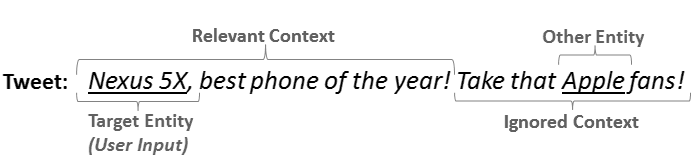
\includegraphics[width=\linewidth]{12_feature_sentence_context}
    \caption{Sentence separation context identification of tweet}
    \label{fig12:feature_sentence_context}
\end{figure}

\pagebreak

\item \textbf{"But" clause}: "But" clause context extraction method is similar to a sentence separation process. Sentences with "but" like clauses (“with the exception of”, “except that” and “except for”) are splinted using as separation point the position of these clauses. \autoref{fig13:but_clause_context} illustrates this idea, for this example only the content to the left side of the token "but" will be extracted an considered for sentiment evaluation. The remaining part of the sentence is irrelevant due to the presence of another entity (no-target).

\end{enumerate}

\begin{figure}[H]
    \centering
    \caption{But clause context extraction of tweet}
    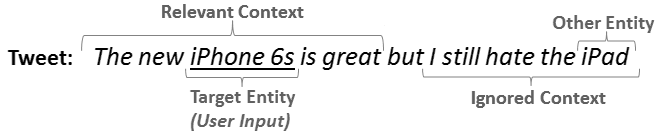
\includegraphics[width=\linewidth]{13_but_clause_context}
    \label{fig13:but_clause_context}
\end{figure}

\subsubsection{Lexicon Features}

After a successful extraction of sentiment contexts, lexical features can be generated from those contexts. Lexicon features are the heart of a sentimentt classifier and usually represent the most effective set of features.  Many different opinion lexicons can be used to represent the numerical sentiment values of tweets. Hence, the classifier presented in this master's thesis combines seven different state-of-the-art sentiment lexicons.  For each of these lexicons, the following set of features is calculated to generate a compelling sentiment feature vector~\cite{MohammadKZ2013}:

\begin{enumerate}
\itemsep0em 

\item \textbf{No. Tokens}: the number of sentiment tokens in the tweet.  These tokens are words with sentiment scores above or below zero in a lexicon.

\item  \textbf{Total Score}: total sentiment score calculated in tweet. 

\item \textbf{Max Score}: highest sentiment score obtained in the tweet.

\item \textbf{Last Token}: sentiment score of last token.

\end{enumerate}

When an entity context has negated tokens, sentiment scores for those tokes are inverted. The solutions presented in this project uses a combination of different lexicons, the quality of these lexicons is critical for the classifier. Therefore, the following state-of-the-art lexical resources were selected for this task:  

\pagebreak

\begin{itemize} 
\itemsep0em  

\item \textbf{MaxDiff}~\cite{kiritchenko2014sentiment}: It is a manually labeled lexicon developed by crowdsourcing and using the MaxDiff method. The lexicon contains 1,500 positive and negative words which are scored from -1 to 0 and 0 to 1.

\item \textbf{Bing Liu}~\cite{hu2004mining}~\cite{liu2005opinion}: Developed by Bing Liu, all terms of this lexicon are manually labeled. It contains 6.790 positive and negative words which are not scored.

\item  \textbf{AFINN}~\cite{nielsen2011new}: Manually labeled lexicon composed by 2.477 words, each word has a sentiment score in the range of -5 to 5. 

\item \textbf{SentiWordNet}~\cite{esuli2006sentiwordnet}: built over WordNet lexical database which contains ~150.000 words. This lexical resource assigns sentiment scores in a range of -1 to 1 with decimal values. Unlike BingLiu and AFINN lexicons, SentiWordNet scores are semi-automatically generated from manually labeled seed-words using  semi-supervised techniques. 

\item \textbf{MPQA}~\cite{wilson2005recognizing}: just like SentiWordNet, MPQA is a subjectivity lexicon created by using semi-supervised techniques. This lexical resource has 6.880 labeled words with no score intensities, only positive and negative.   

\item \textbf{NRC Hashtag / Sentiment140}~\cite{NRCJAIR14}: Developed by Mohammad Saif, both lexicons were generated fully automatically with distant supervision techniques. NRC Hashtag and Sentiment 140 lexicons contain 54,129 and 62,468 words respectively. Both represent the sentiment value of words with scores between -$\infty$ (most negative) to $\infty$ (most positive).


\end{itemize}

\begin{table}[H]
\centering
\caption{Lexical resources summary.}
\label{tab:lexical_resources}
\begin{tabular}{|l|c|c|}
\hline
\multicolumn{1}{|c|}{\textbf{Lexicon}} & \textbf{Score Range} & \textbf{No. Words} \\ \hline
MaxDiff Twitter                        & Real-values          & 1,500              \\ \hline
AFINN                                  & -5 to 5              & 2,477              \\ \hline
BingLiu                                & Pos / Neg            & 6,785              \\ \hline
SentiWordNet                           & -1 to 1              & 147,292            \\ \hline
MPQA                                   & Pos / Neg            & 6,886              \\ \hline
NRC Hashtag                            & Real-values          & 54,129             \\ \hline
Sentiment140                           & Real-values          & 62,468             \\ \hline
\end{tabular}
\end{table}

\pagebreak

\subsubsection{Emoticon Features}

The informal nature of tweets is characterized by the common usage of emoticons to express sentiment. Therefore, emoticons are also considered for the generation of feature vectors. Only those emoticons contained on the target-entity context are used to generate this features. The vector composition is fairly simple: \textit{No. of positive emojis (e.g. ":)", ":D", ";)" ) / No. of negative emojis (e.g. ":(", "D:")}.

In \autoref{tab:entity_vectors} an example of entity-based feature vectors is presented. Notice that there is only one emoticon in the example and it has positive value, hence the result vector is {1,0} (+1 positive, 0 negative). Similar rules apply to BingLiu lexicon features, two positive words in the tweet with no negative sentiments. 

\begin{table}[H]
\centering
\caption{Entity-based feature vectors example}
\label{tab:entity_vectors}
\begin{tabular}{l|l}
\multicolumn{1}{c|}{{\color[HTML]{000000} \textbf{Target-entity context tokens}}}                                         & \multicolumn{1}{c}{{\color[HTML]{000000} \textbf{Feature Vectors}}}                                     \\ \hline
{\color[HTML]{000000} \begin{tabular}[c]{@{}l@{}}\{my, TargetEntity, is, {\color[HTML]{036400}awesome}, \\ {\color[HTML]{036400}best}, day, ever, {\color[HTML]{036400}:D} \}\end{tabular}} & {\color[HTML]{000000} \begin{tabular}[c]{@{}l@{}}(BingLiu)\{2, 2, 1, 1\}\\ (Emoji)\{1,0\}\end{tabular}}
\end{tabular}
\end{table}

\section{Support Vector Machine}

This component represents the final stage of proposed sentiment classification solution. There are many supervised learning models such as Maximum Entropy, Naive Bayes and Neural Networks. However, Support Vector Machines (SVMs) have the potential to handle large feature spaces in a very efficient way~\cite{joachims1998text}. Hence, a SVM is used to deal with the large set of features generated from tweets and entities, the generation of this features is explained in \autoref{sec:feature_generation}. Like any other supervised learning model, SVMs require training data to function. This training data is represented as numerical feature vectors labeled with their respective class, the labeling process is usually done manually (by evaluators) but in some cases distant-supervision methods are used. The job of any SVM is to find a clear separation between training vectors and their classes, based on this learning process, the SVM is able to classify new document entries (tweets for this case). 

Proposed entity-based classifier uses a support vector machine (SVM) NodeJS module called \textit{Node-SVM} which is a port from the C++ SVM library \textit{LIBSVM}~\cite{chang2011libsvm}. This library is one of the most popular SVM solutions available for machine learning based classification and regression. To have a better understanding of implemented classifier, the parameters used to setup \textit{Node-SVM} are the following:

\begin{itemize} 
\itemsep0em  

\item \textbf{SVM Type:} C-Support Vector Classification (C\_SVC). n-class classification where n $>$ 2, allows multi-class classification (positive, negative and neutral).

\item  \textbf{Kernel}: Default Liner kernel is used.  

\item  \textbf{Normalization}: During SVM data pre-processing, mean normalization is required.  

\item  \textbf{Shrinking}: Usage of shrinking heuristics.  

\item  \textbf{Probability}: Disable the usage of probability estimates.  

\end{itemize}

\autoref{fig15:linear_svm} illustrates the linear form of a SVM which is a hyperplane that divides a set of positive data points (positive labeled tweets) from a set of negative data points. The separation distance between these two set is called \textit{maximum margin}. In linear SVMs, the maximum margin represents the maximum distance of the hyperplane to the positive and negative data points. 

\begin{figure}[H]
    \centering
    \caption[Illustration of a linear Support Vector Machine]{Illustration of a linear Support Vector Machine{~\cite{platt1998sequential}}}
    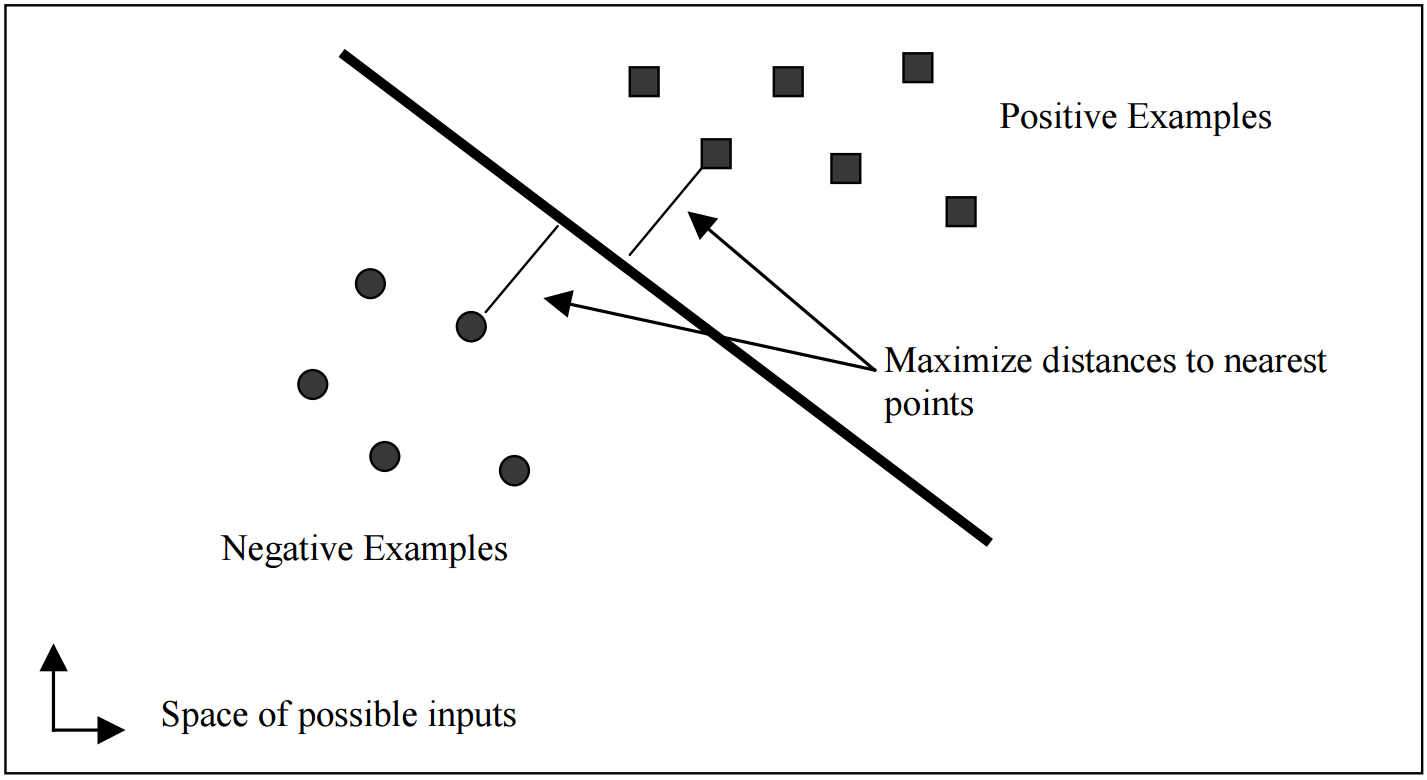
\includegraphics[width=\linewidth]{15_linear_svm}
    \label{fig15:linear_svm}
\end{figure}


\section{SentiTrack Integration}

For a full description of the SentiTrack system refer to \autoref{sec:sentitrack}. The integration process of the sentiment classifier developed in this master's thesis and the SentiTrack system was fairly simple since both platforms are fully developed with NodeJS (JavaScript) technologies. Therefore, in order to perform the integration, the proposed classifier was implemented as a NodeJS module using the JS package manager (npm) approach. \autoref{fig16:package_files} shows the package organization of implemented module (source code files), the name of the module is \textit{entity\_sentiment} which refers to the capabilities of implemented entity-based sentiment classifier. The following line of code is required to make use of the \textit{entity\_sentiment} module:

 \begin{displayquote}
var entitysentiment = require("entity\_sentiment");
\end{displayquote} 

This line will allow NodeJS classes to perform classification using proposed solution. In following \autoref{sec:evaluation} the quality and performance of developed classifier is tested and evaluated, then an analysis of result is presented. 

\begin{figure}[H]
    \centering
    \caption[Package files organization]{Package files organization}
    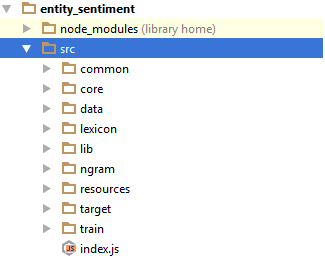
\includegraphics[width=9cm,height=13cm,keepaspectratio]{16_package_files}
    \label{fig16:package_files}
\end{figure}
  % Ontology re-use

\chapter{Evaluation and Analysis of Results}
\label{sec:evaluation}

This chapter presents the evaluation and results of the entity-based sentiment classifier developed in this master's thesis. The chapter is divided in three sections. First one, describes the process of collecting the datasets used to train the classifier and evaluate the proposed solution. The second section is about quality evaluation,  here the overall success of the implemented sentiment classifier is tested and analyzed. Finally, the performance of the classifier is measured and compared with other similar solutions. 

\section{Data Collection and Processing}
\label{sec:collection}

Sentiment classifiers that make use of machine learning methods require a corpus of labeled documents as training data in order to function. Usually the data is manually labeled by evaluators. However, the level of sentiment classification will determine which type of training data is necessary. For sentiment analysis of tweets, these are the most used types of datasets:

\begin{itemize} 
\itemsep0em  

\item \textbf{Document-level}: Documents are labeled based on the sentiment orientation expressed in the whole tweet span without considering the presence of entities or differentiation between expressions. This is the most common type of Twitter sentiment corpus, but it is not useful for an entity based sentiment classifier.

\item \textbf{Entity-level}: Unlike document-level training data, entity-based labeled corpus must reflect the sentiment expressed towards a given entity or query. \autoref{tab:twitter_corpus} shows how the dataset is organized.

\end{itemize}

\begin{table}[H]
\centering
\caption{Entity-based Twitter corpus example.}
\label{tab:twitter_corpus}
\begin{tabular}{|l|c|c|}
\hline
\multicolumn{1}{|c|}{\textbf{Sentiment}} & \textbf{Query/Target} & \textbf{Tweet}                                                                                                                            \\ \hline
Positive                                 & apple                 & \begin{tabular}[c]{@{}c@{}}I'm lovin the iPhone update especially the slide \\ down bar at top of screen =) good job @Apple.\end{tabular} \\ \hline
Negative                                 & twitter               & \begin{tabular}[c]{@{}c@{}}\#Twitter are you freaking kidding me \\ \#wth... http://t.co/zKn2bu5R\end{tabular}                            \\ \hline
Neutral                                  & microsoft             & \begin{tabular}[c]{@{}c@{}}Developers: Let Microsoft Market Your App \\ for Windows Phone http://t.co/QZUqhCxx\end{tabular}               \\ \hline
\end{tabular}
\end{table}

For the development and evaluation of presented entity-based sentiment classifier, a collection of several entity-based labeled corpus was created. This collection is composed by the following datasets:

\begin{itemize} 
\itemsep0em  

\item \textbf{Sanders Analytics\footnote{\url{http://www.sananalytics.com/lab/twitter-sentiment/
}}}:  this dataset is for training and testing sentiment analysis algorithms. It is composed by 5513 manually classified tweets. A 3-class classification method was used (positive, negative, neutral) and each tweet expresses sentiment towards a specific entity.  

\item \textbf{STS-Gold\footnote{\url{http://tweenator.com/index.php?page_id=13
}}}~\cite{saif2013evaluation}: Developed by Mohammad Saif, is a dataset where tweets and targets (entities) are annotated individually. Therefore, only the opinions expressed towards those entities is relevant for result labels.

\item \textbf{SemEval 2015 / 2016}~\cite{rosenthal2015semeval}: SemEval (Semantic Evaluation) is an event held every year where new semantic analysis systems are evaluated. Teams from universities and institutions around the globe submit their solutions to a set of problem tasks defined by the competition committee. One of these task is about Twitter sentiment analysis, therefore, SemEval provides labeled datasets that allow participants to train and evaluate their sentiment classifiers.


\end{itemize}

A normalization process was necessary to remove repeated tweets and noisy tokens from the collection, additionally, a balance between the three different sentiment classes (positive, negative, and neutral) had to be achieve in order to guarantee effective performance of the support vector machine. As a result, \autoref{tab:datasets_summary} shows a summary of the collected tweets. 70\% of the 4900 labeled tweets is used as training data leaving a 30\% for evaluation and testing porpoises. 

\begin{table}[H]
\centering
\caption{Datasets Summary}
\label{tab:datasets_summary}
\begin{tabular}{|l|c|c|c|c|}
\hline
\multicolumn{1}{|c|}{{\color[HTML]{000000} \textbf{Dataset}}} & {\color[HTML]{000000} \textbf{No. of Tweets}} & \textbf{\#Negative} & \textbf{\#Neutral} & \textbf{\#Positive} \\ \hline
{\color[HTML]{000000} Sanders Analytics}                      & {\color[HTML]{000000} 5513}                   & 654                 & 2503               & 570                 \\ \hline
STS-Gold                                                      & 498                                           & 177                 & 139                & 192                 \\ \hline
SemEval 2016                                                  & 2825                                          & 862                 & 965                & 998                 \\ \hline
SemEval 2015                                                  & 1105                                          & 213                 & 422                & 470                 \\ \hline
Normalization                                                 & 4900                                          & 1634                & 1633               & 1633                \\ \hline
\end{tabular}
\end{table}


\section{Quality Evaluation}
In order to measure the quality of the entity-based sentiment classifier developed in this master's thesis, standard evaluation metrics were considered. Therefore, both correct and incorrect predictions must be measured to calculate aforementioned metrics. \autoref{tab:confusion_matrix} presents a three-class confusion matrix which is used to visualize the level of accuracy of predicted data against test datasets.   


\begin{table}[H]
\centering
\caption{3-Class Confusion Matrix}
\label{tab:confusion_matrix}
\begin{tabular}{|l|c|c|c|}
\hline
\multicolumn{1}{|c|}{{\color[HTML]{000000} \textbf{Data Class}}} & {\color[HTML]{000000} \textbf{Classified as Pos}} & \textbf{Classified as Neg} & \textbf{Classified as Neu} \\ \hline
{\color[HTML]{000000} \textbf{Positive}}                         & {\color[HTML]{036400} true positive}              & false negative             & false neutral              \\ \hline
\textbf{Negative}                                                & false positive                                    & {\color[HTML]{036400} true negative}              & false neutral              \\ \hline
\textbf{Neutral}                                                 & false positive                                    & false negative             & {\color[HTML]{036400} true neutral}               \\ \hline
\end{tabular}
\end{table}

Using the confusion matrix illustrated in \autoref{tab:confusion_matrix}, several different metrics were calculated for the evaluation of the classifier. The scoring metrics considered in this project are the following:

\begin{itemize} 
\itemsep0em  

\item \textbf{Precision}: Precision is the rate of correct predictions over the universe of predictions (true + false). For the positive class, precision is defined as follows:
    
    \begin{equation}
        precision = \frac{\text{true positive}}{\text{true positive} + \text{false positive}} 
    \end{equation}
    
\item \textbf{Recall}: is the fraction of relevant tweets that are successfully predicted.  Continuing with positive class example, recall is defined as:

    \begin{equation}
        recall = \frac{\text{true positive}}{\text{true positive} + \text{false negative} + \text{false neutral}} 
    \end{equation}
    
\item \textbf{Accuracy}: is an overall representation of correct predictions. For a three-class classifier, it is defined as follows:

    \begin{equation}
        accuracy = \frac{\text{total correct prediction}}{\text{total correct prediction} + \text{total incorrect prediction}} 
    \end{equation}

\item \textbf{F-Score}: (F-Measure) is defined as the combination of precision and recall. This is the result formula for class \textit{positive}:

    \begin{equation}
        Fscore = 2 * \frac{precision_{positive} * recall_{positive}}{precision_{positive} + recall_{positive}} 
    \end{equation}

\end{itemize}

Based on 4900 collected tweets (datasets) and previews described metrics, a 4-fold cross validation test was performed in proposed entity-based sentiment classifier. The results are presented in \autoref{tab:first_results}. According to obtained results, proposed classifier achieved an accuracy of 0.635 (64\%).
\begin{table}[H]
\centering
\caption{Precision, Recall and F-Score results}
\label{tab:first_results}
\begin{tabular}{l|c|c|c}
\hline
\multicolumn{1}{|c|}{{\color[HTML]{000000} \textbf{Data Class}}} & {\color[HTML]{000000} \textbf{Precision}} & \textbf{Recall} & \multicolumn{1}{c|}{\textbf{Fscore}} \\ \hline
\multicolumn{1}{|l|}{{\color[HTML]{000000} Positive}}            & {\color[HTML]{000000} 0.594}              & 0.668           & \multicolumn{1}{c|}{0.629}           \\ \hline
\multicolumn{1}{|l|}{Negative}                                   & 0.650                                     & 0.615           & \multicolumn{1}{c|}{0.632}           \\ \hline
\multicolumn{1}{|l|}{Neutral}                                    & 0.669                                     & 0.622           & \multicolumn{1}{c|}{0.645}           \\ \hline
Total:                                                           & 0.637                                     & 0.635           & 0.635                               
\end{tabular}
\end{table}

Results in \autoref{tab:first_results} show that the class \textit{positive} achieved the lowest performance while \textit{neutral} class obtained the highest. \textit{Neutral} class tends to get better results since its classification depends on the absence of sentiment expressions. Therefore, polarity classification represents a bigger challenge because of possible presence of negation context and sarcasm comments.

\subsection{Features Contribution}

As explained in \autoref{sec:feature_generation}, the generation of feature vectors is an essential process for sentiment classifiers. Hence, the contributions made by each of the features generated for proposed classifier are illustrated in \autoref{tab:contributions} and \autoref{fig17:contributions_graph}. 

\begin{table}[H]
\centering
\caption{Features contribution details}
\label{tab:contributions}
\begin{tabular}{l|l|l|l|l}
\multicolumn{1}{c|}{{\color[HTML]{000000} \textbf{}}} & \textbf{F-Score} & \textbf{Accuracy} & \textbf{Diff-F} & \textbf{Diff-A} \\ \hline
{\color[HTML]{000000} \textbf{All Features}}          & 0.629            & 0.635             &                 &                 \\ \hline
/ - Unigrams                                          & 0.619            & 0.626             & - 0,01          & - 0,009         \\ \hline
/ - Emoticons                                         & 0.618            & 0.626             & - 0,01          & - 0,009         \\ \hline
/ - Content                                           & 0.536            & 0.571             & - 0,093         & - 0,064         \\ \hline
/ - POS Tags                                          & 0.541            & 0.576             & - 0,088         & - 0,059         \\ \hline
/ - Lexicon                                           & 0.362            & 0.495             & - 0,267         & - 0,14          \\ \hline
\end{tabular}
\end{table}

\begin{figure}[H]
    \centering
    \caption[Features Contribution Graph]{Feature Contributions Graph}
    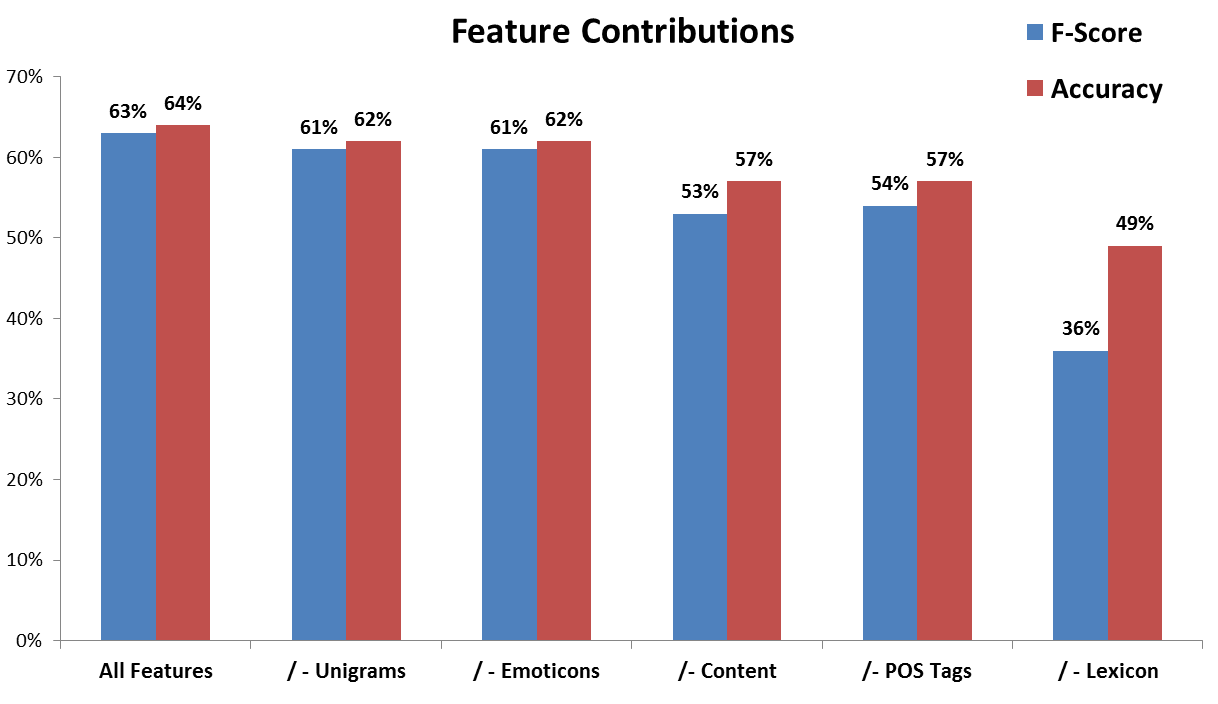
\includegraphics[width=\linewidth]{17_contributions_graph}
    \label{fig17:contributions_graph}
\end{figure}

These results show how important the lexicon features are to the overall performance of the classifier, the contribution of the seven state-of-the-art lexical resources is significantly higher than the contributions obtained by other features. Content and POS Tags features achieved very interesting results surpassing unigrams and emoticons features by a considerable margin. Although unigrams and bag-of-words are some of the most popular features, the evaluation results yield insignificant contributions from this vector. Therefore, its possible to assume that in an entity-based classification approach, n-grams might not have the same contribution impact as in document-level sentiment classifiers.   

\subsection{Quality Comparison}

In order to extend the evaluations made to proposed sentiment classifier, a performance comparison between this master's thesis solution and two additional sentiment classification tools was made. The following tools were considered: 

\begin{itemize} 
\itemsep0em  

\item \textbf{Former SentiTrack Classifier}: SentiTrack as described in \autoref{sec:sentitrack} requires a sentiment classifier to project public's opinion about specific companies in Twitter. Proposed sentiment classifier aims to replace the already existing classifier which is referred as \textit{former SentiTrack classifier}. Former classifier uses unsupervised techniques such as lexicons and linguistic rules to classify tweets as positive, negative or neutral. Also, it is based on a very popular NodeJS module called \textit{Sentiment}\footnote{\url{https://www.npmjs.com/package/sentiment}}. 

\item \textbf{CompendiumJS\footnote{\url{https://github.com/Ulflander/compendium-js}}}: is a suit of natural language processing tools for NodeJS platform. This module provides a lexicon-based sentiment classifier capable of perform three-class classification. 

\end{itemize}

\begin{figure}[H]
    \centering
    \caption[Classifiers Comparison Graph]{Classifiers Comparison Graph}
    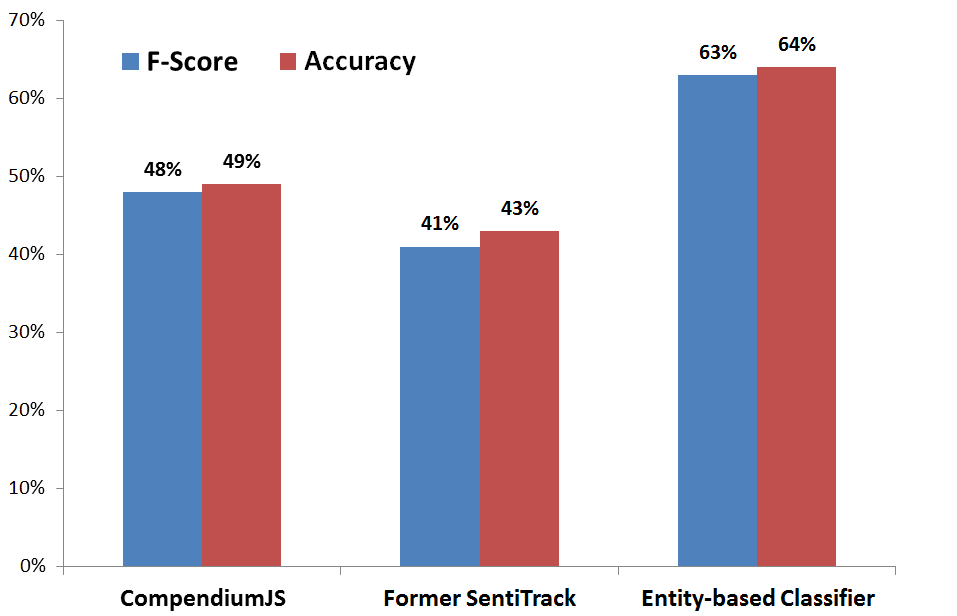
\includegraphics[width=\linewidth]{18_comparison_graph}
    \label{fig18:comparison_graph}
\end{figure}

\autoref{fig18:comparison_graph} illustrates the results obtained by a 4-fold cross validation test of 4900  target-labeled tweets (\autoref{sec:collection}) performed over three sentiment classifiers including the one developed and proposed in this master's thesis. The results show a significant difference in F-Score and Accuracy between the entity-based classifier and the other two tools. Former SentiTrack classifier's poor performance is consequence of its simplicity, it is based on one single lexical resources \textit{AFINN} with no consideration of negation context and emoticons. The difference between results is related to the classification techniques, most state-of-the-art sentiment classifiers for Twitter use supervised methods capable of analyze many tweet-specific features. Hence, presented solution make use of machine learning methods.  


\section{Performance Evaluation}

A performance evaluation measures how long will take proposed classifier to process a given amount of tweets. This is a very important evaluation given that one of the objectives of this research project is to develop a sentiment classifier capable of function under real-time processing systems such as SentiTrack. Additionally, the performance test is also done to former SentiTrack classifier and CompendiumJS in order to compare resulting processing times. These are the evaluation environment specifications: 

\begin{itemize} 
\itemsep0em  

\item \textbf{Processor}: Intel Core i5-2320 CPU @ 3.00GHz

\item \textbf{Memory RAM}: 8 GB 

\item \textbf{Operative System}: 64 bits Windows 7

\end{itemize}

The results are shown in \autoref{tab:performance_results}, they reflect a large difference in performance time between former SentiTrack classifier and proposed solution. Can be inferred, that the complex pipeline of processes required by the entity-based classifiers and the usage of supervised techniques have an impact in classification time. However, the performance achieved by proposed solution is good enough to cope with real-time processing enviroments like SentiTrack.  

\begin{table}[H]
\centering
\caption{Performance test results}
\label{tab:performance_results}
\begin{tabular}{l|c}
\multicolumn{1}{c|}{{\color[HTML]{000000} \textbf{}}} & \textbf{1000 Tweets} \\ \hline
{\color[HTML]{000000} \textbf{Entity-based (ms)}}     & 3447.054             \\ \hline
\textbf{Former SentiTrack (ms)}                       & 323.310              \\ \hline
\textbf{CompendiumJS (ms)}                            & 2357.886             \\ \hline
\end{tabular}
\end{table}

\section{SentiTrack Experiment}

After proposed/built entity-based sentiment classifier was integrated to SentiTrack, an experiment was performed. This experiment intends to find a correlation between the two variables (social media sentiment, stock market prices) filtering and classifying live tweets; as well as stock market movements, over a week for a set of 6 companies. Moreover, a correlation test was done over collected sentiments and stock market data for each evaluated company. 

The overall results were very positive in comparison to previews SentiTrack experiments where the former classifier was used, evidence of a moderate correlation was found on 3 out of 6 companies with a maximum correlation of 0.84 (84\%). These results prove a successful integration between proposed/built sentiment classifier and SentiTrack, which will provide a more accurate analysis for future experiments. 


 % Smart Service in use

\chapter{Conclusions and Future Work}
\label{sec:conc} 

This thesis presented the research, evaluation and solution for an entity-based sentiment classifier for social media analysis. Implemented system is able to perform sentiment classification of tweets based on the presence of entities and the opinion expressions targeting them. 

This chapter aims conclude this masters thesis project with a summary of the achievements made, limitations encountered and possible future extensions and enhancements. 



\section{Achievements}

\begin{itemize} 
\itemsep0em  

\item The main goal of this thesis is the study of an entity-based sentiment classification approach for the analysis of social media data. The research presents the facts, reasons and evaluation results that led the project to the usage of most suitable methods for required solution.

\item A successful approach was produced for the required solution. The presented approach is able to extract opinion expressions aiming relevant entities in tweets.

\item The solution achieved satisfactory result in terms of Accuracy and F-Score, surpassing by a significant margin evaluated alternatives for sentiment classification.

\item In terms of performance time, developed classifier is capable of work under real-time processing systems.

\item Presented solutions was successfully integrated to SentiTrack, providing an improved sentiment analysis experience.

\item The clean organization and structure of developed system, allows future interested researches to improve and modify provided tools.



\end{itemize}

\section{Limitations}

\begin{itemize} 
\itemsep0em  

\item Memory issues limited the development of the classifier to the use of unigrams with bag-of-word method. The usage of different levels of n-grams as features might have contributed significantly with better final results.

\item Some NodeJS modules used by developed classifier may produce incompatibility errors in specific versions of Windows OS, this issue is related to the usage of c++ libraries and other native resources.

\item Despite the fact that entity-targeted opinion expressions were extracted from tweets, there are many cases where no clear separation of sentence is made, leading to incorrect classifications.  

\item Presented solution is unable of identify the presence of advertisements and sarcasms in tweets. Therefore, sentiment analysis of specific products may yield inconsistent results.  


\end{itemize}

\section{Future Work}

\begin{itemize} 
\itemsep0em  

\item An expansion of the sentiment classifier with a dependency parser capable of perform under real-time systems, would improve considerably the accuracy of the solution.   

\item Improvements in accuracy can be made by using a more accurate named entity recognition module and higher levels of n-grams as feature vectors.

\item Performance of the system could be enhanced by exploring the usage of different POS tagging solutions and automatic tokenization libraries.  

\item Extend the solution to work with other social networks such as Facebook, LinkedIn and Google plus.  


\end{itemize} % Conclusions and Future Work

%% ----------------------------------------------------------------

% Now begin the Appendices, including them as separate files

\addtocontents{toc}{\vspace{2em}} % Add a gap in the Contents, for aesthetics

\appendix % Cue to tell LaTeX that the following 'chapters' are Appendices

%% Appendix A

\chapter{Namespaces} % Main appendix title

\label{appendix:Namespaces} % For referencing this appendix elsewhere, use \ref{AppendixA}

	% Appendix Title

%\chapter{Appendix}
\label{sec:App} 

\section{Glossary}


\begin{table}[H]
\centering
\label{my-label}
\begin{tabular}{|c|l|}
\hline
\textbf{Blog}      & Abbreviation to WebLog                                                                                                            \\ \hline
\textbf{Emoticon}  & Short for emotion icon. e.g. ":D", ":)", ":-)"                                                                                    \\ \hline
\textbf{Hashtag}   & Topic labels used in Twitter posts.                                                                                               \\ \hline
\textbf{Microblog} & \begin{tabular}[c]{@{}l@{}}Sites where users express their ideas in the form of\\ small units of text. e.g. Twitter.\end{tabular} \\ \hline
\textbf{Tweet}     & Short message or post.                                                                                                            \\ \hline
\textbf{SO}        & Sentiment Orientation                                                                                                             \\ \hline
\textbf{NLP}       & natural language processing                                                                                                       \\ \hline
\textbf{Lexicon}   & Dicctionary or lexical resource                                                                                                   \\ \hline
\end{tabular}
\end{table}

\clearpage

\section{Technical Specifications}

The source code of the project can be downloaded from the following link which points to
the Git repository of the EIS group, University of Bonn. 

\textbf{Link to thesis repository: }

https://github.com/EIS-Bonn/Theses/tree/master/2015/Cristobal\_Leiva

To run the application, the system has to fulfill the following requirements and the user
needs to follow the instructions given below.

\textbf{Requirements:}

\begin{itemize} 
\itemsep0em  

\item Node.js + NPM

\item Latest MongoDB

\item Bower (get by running "npm install -g bower")

\item Gulp (get by running "npm install -g gulp")


\end{itemize}

\textbf{How to Install:}

\begin{enumerate} 
\itemsep0em  

\item Install the required NodeJS modules: npm install

\item Configure Twitter API keys: pen config.sample.js and fill in the required keys under the twitter app
config and save it as config.js

\item To start NodeJS server: start mongo then run the command "gulp"

\item Run the web browser: http://localhost:8082/resa


\end{enumerate}

\clearpage
\section{SentiTrack GUI}

\begin{figure}[H]
    \centering
    \caption{SentiTrack front-end, bubble cloud}
    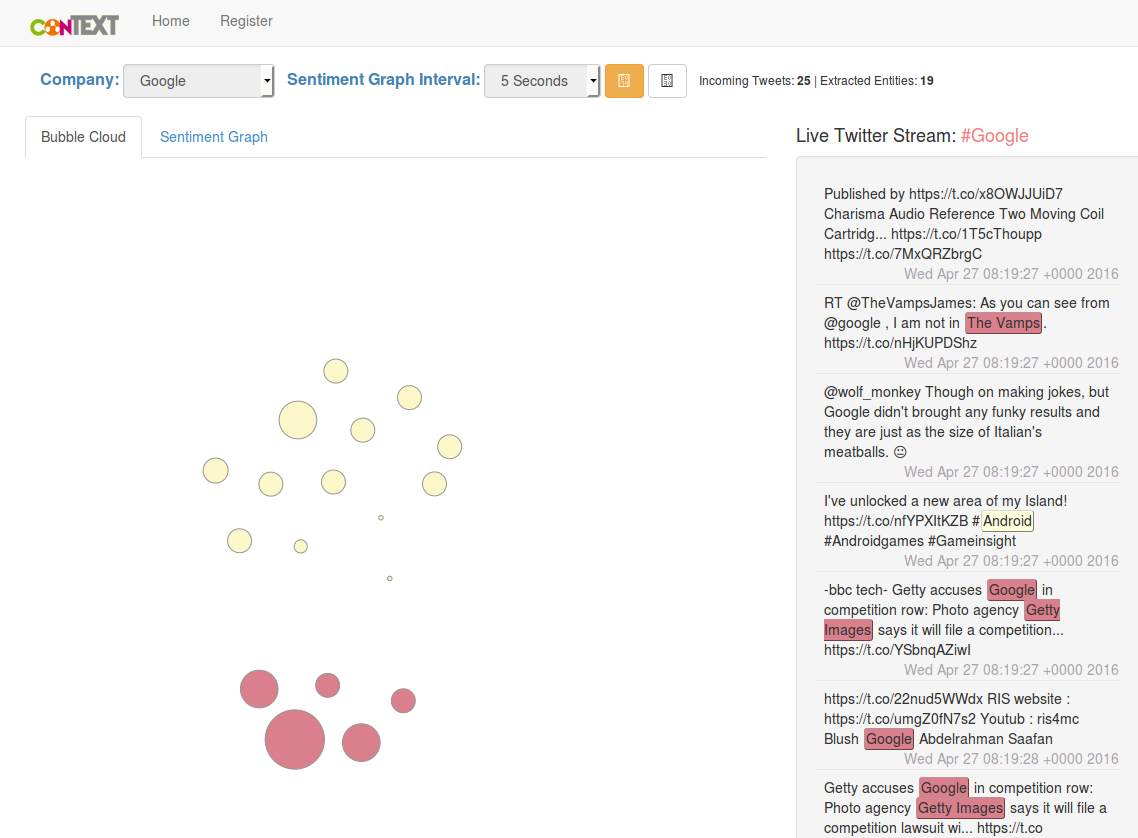
\includegraphics[width=\linewidth]{19_sentitrack_01}
    \label{}
\end{figure}

\begin{figure}[H]
    \centering
    \caption{SentiTrack front-end, live sentiment data}
    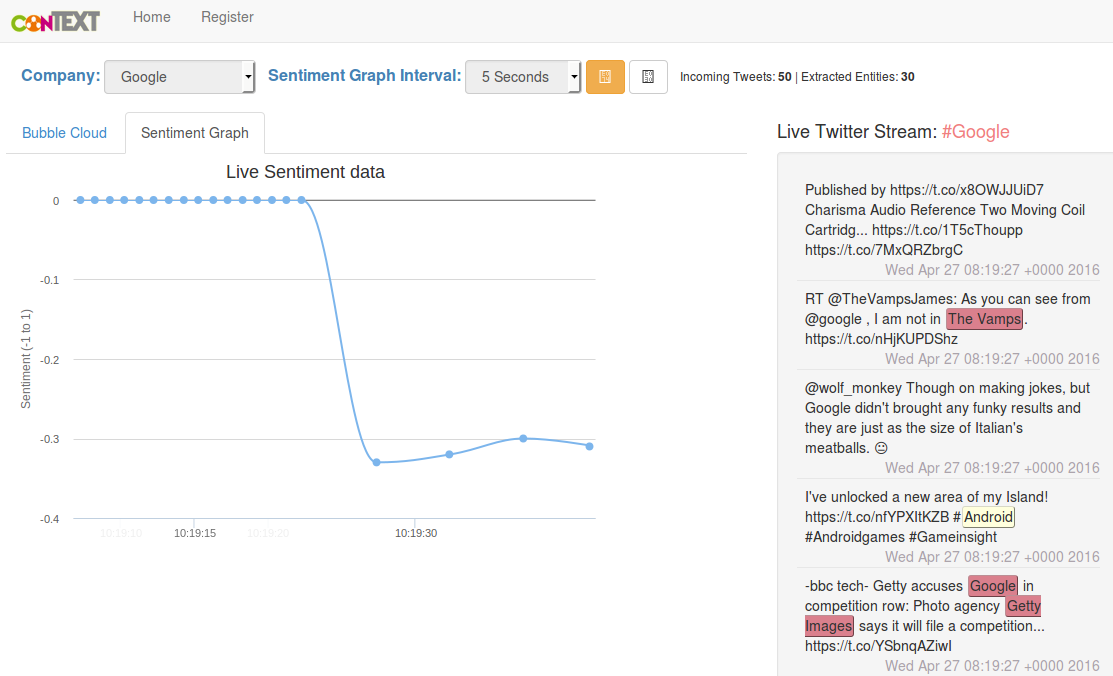
\includegraphics[width=\linewidth]{20_sentitrack_02}
    \label{}
\end{figure}
 % Appendix Title

%\input{Appendices/AppendixC} % Appendix Title

\chapter{Appendix}
\label{sec:App} 

\section{Glossary}


\begin{table}[H]
\centering
\label{my-label}
\begin{tabular}{|c|l|}
\hline
\textbf{Blog}      & Abbreviation to WebLog                                                                                                            \\ \hline
\textbf{Emoticon}  & Short for emotion icon. e.g. ":D", ":)", ":-)"                                                                                    \\ \hline
\textbf{Hashtag}   & Topic labels used in Twitter posts.                                                                                               \\ \hline
\textbf{Microblog} & \begin{tabular}[c]{@{}l@{}}Sites where users express their ideas in the form of\\ small units of text. e.g. Twitter.\end{tabular} \\ \hline
\textbf{Tweet}     & Short message or post.                                                                                                            \\ \hline
\textbf{SO}        & Sentiment Orientation                                                                                                             \\ \hline
\textbf{NLP}       & natural language processing                                                                                                       \\ \hline
\textbf{Lexicon}   & Dicctionary or lexical resource                                                                                                   \\ \hline
\end{tabular}
\end{table}

\clearpage

\section{Technical Specifications}

The source code of the project can be downloaded from the following link which points to
the Git repository of the EIS group, University of Bonn. 

\textbf{Link to thesis repository: }

https://github.com/EIS-Bonn/Theses/tree/master/2015/Cristobal\_Leiva

To run the application, the system has to fulfill the following requirements and the user
needs to follow the instructions given below.

\textbf{Requirements:}

\begin{itemize} 
\itemsep0em  

\item Node.js + NPM

\item Latest MongoDB

\item Bower (get by running "npm install -g bower")

\item Gulp (get by running "npm install -g gulp")


\end{itemize}

\textbf{How to Install:}

\begin{enumerate} 
\itemsep0em  

\item Install the required NodeJS modules: npm install

\item Configure Twitter API keys: pen config.sample.js and fill in the required keys under the twitter app
config and save it as config.js

\item To start NodeJS server: start mongo then run the command "gulp"

\item Run the web browser: http://localhost:8082/resa


\end{enumerate}

\clearpage
\section{SentiTrack GUI}

\begin{figure}[H]
    \centering
    \caption{SentiTrack front-end, bubble cloud}
    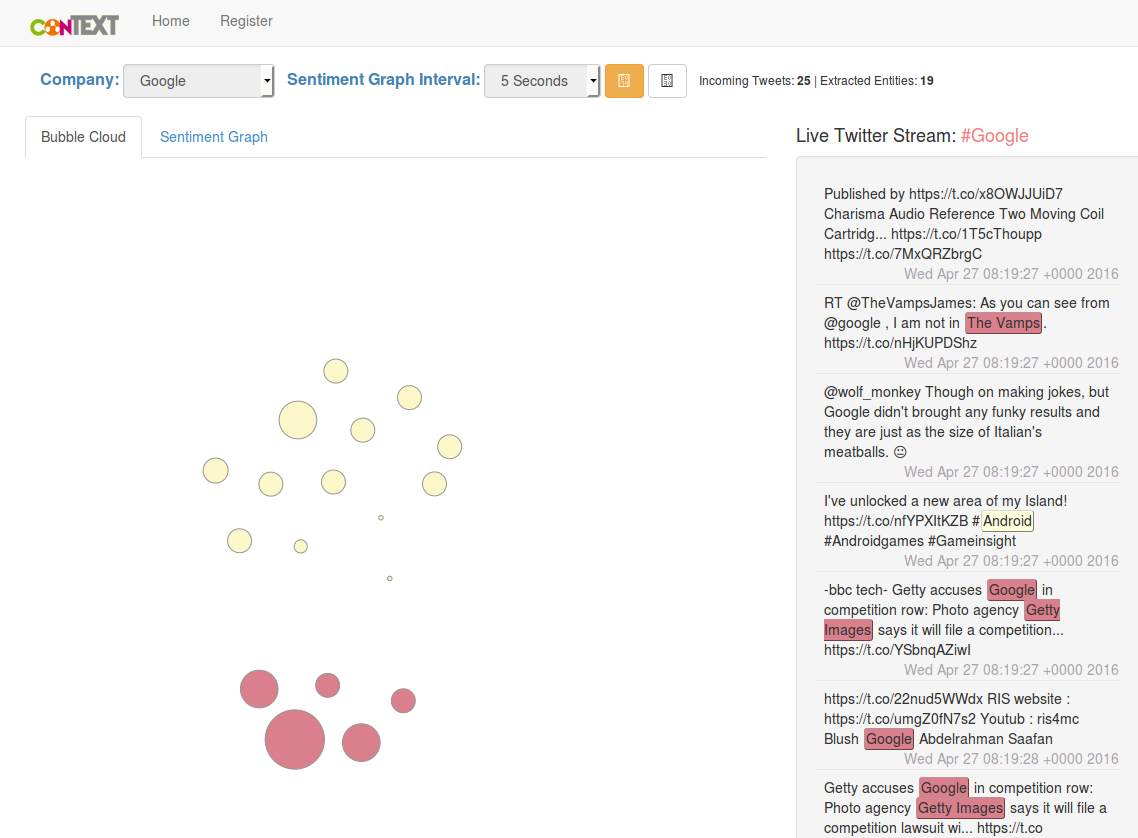
\includegraphics[width=\linewidth]{19_sentitrack_01}
    \label{}
\end{figure}

\begin{figure}[H]
    \centering
    \caption{SentiTrack front-end, live sentiment data}
    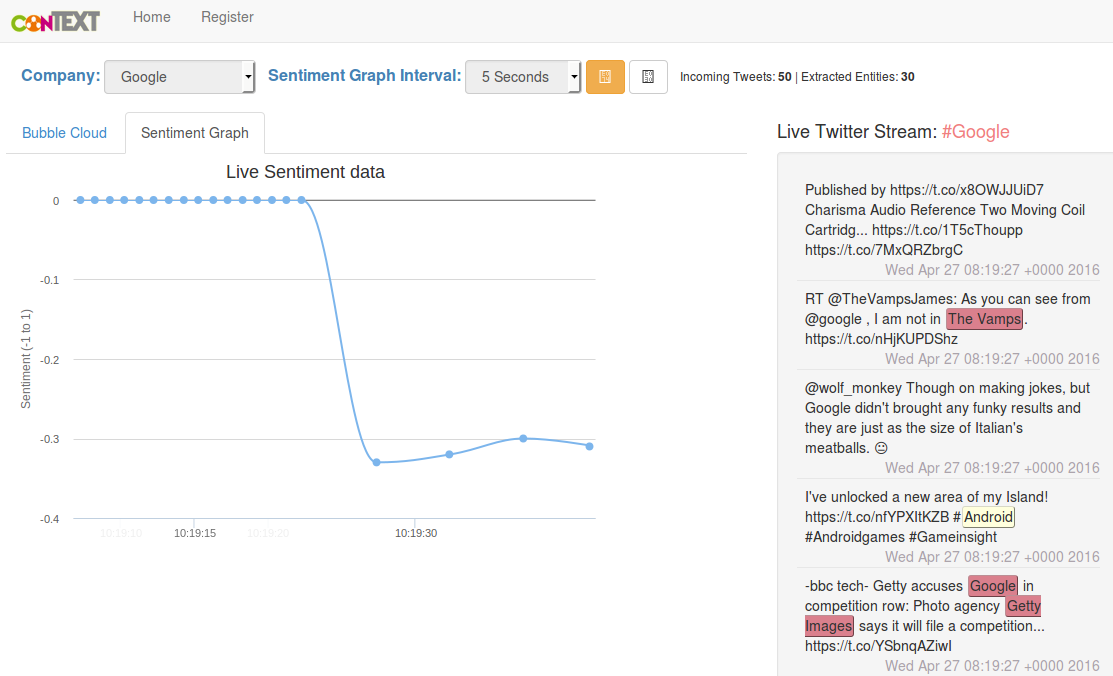
\includegraphics[width=\linewidth]{20_sentitrack_02}
    \label{}
\end{figure}
 % Appendix Title


\addtocontents{toc}{\vspace{2em}}  % Add a gap in the Contents, for aesthetics
\backmatter

%% -------------------------------------------------------------- ----------------------------------------------------------------
\label{Bibliography}
\lhead{\emph{Bibliography}}  % Change the left side page header to "Bibliography"
\bibliographystyle{unsrtnat}  % Use the "unsrtnat" BibTeX style for formatting the Bibliography
\bibliography{literature}  % The references (bibliography) information are stored in the file named "Bibliography.bib"

\end{document}  % The End
%% ----------------------------------------------------------------